\documentclass[12pt,a4paper]{ctexart}

% ============================================================
% 宏包加载
% ============================================================
\usepackage{amsmath,amssymb,amsthm}
\usepackage{mathrsfs}
\usepackage{graphicx}
\usepackage{booktabs}
\usepackage{tabularx}
\usepackage{multirow}
\usepackage{float}
\usepackage{hyperref}
\usepackage{cite}
\usepackage{algorithm}
\usepackage{algorithmic}
\usepackage{listings}
\usepackage{xcolor}
\usepackage{geometry}
\usepackage{caption}
\usepackage{subcaption}
\usepackage{enumitem}
\usepackage{fancyhdr}
\usepackage{titlesec}

% ============================================================
% 页面设置
% ============================================================
\geometry{left=2.5cm, right=2.5cm, top=2.5cm, bottom=2.5cm}
\setlength{\parindent}{2em}
\setlength{\parskip}{0.5em}

% ============================================================
% 定理环境
% ============================================================
\newtheorem{theorem}{定理}[section]
\newtheorem{lemma}[theorem]{引理}
\newtheorem{proposition}[theorem]{命题}
\newtheorem{corollary}[theorem]{推论}
\newtheorem{definition}{定义}[section]
\newtheorem{remark}{注}[section]

% ============================================================
% 代码样式
% ============================================================
\lstset{
  language=Python,
  basicstyle=\small\ttfamily,
  keywordstyle=\color{blue},
  commentstyle=\color{gray},
  stringstyle=\color{red},
  numbers=left,
  numberstyle=\tiny\color{gray},
  frame=single,
  breaklines=true,
  captionpos=b
}

% ============================================================
% 超链接设置
% ============================================================
\hypersetup{
  colorlinks=true,
  linkcolor=blue,
  citecolor=blue,
  urlcolor=blue
}

% ============================================================
% 标题信息
% ============================================================
\title{\textbf{矩形区域上 Poisson/Helmholtz 方程的 \\ FFT 快速求解器与迭代法对比研究}}
\author{作者姓名 \\ 指导教师：导师姓名\ 教授}
\date{\today}

% ============================================================
\begin{document}

\maketitle

\begin{abstract}
本文在统一的 $(-\nabla^2 + \sigma)u = f$ 框架下，
研究矩形区域上 Poisson 方程（$\sigma=0$）、modified Helmholtz 方程（$\sigma=+\kappa^2$）
与 true Helmholtz 方程（$\sigma=-\kappa^2$）的快速数值求解方法。
首先基于五点差分格式（二阶精度）和九点紧致差分格式（四阶精度）对方程进行离散，
然后利用离散 Fourier 变换（DST/DCT）的对角化性质，实现了 Fourier Analysis (FA)、
Cyclic Reduction (CR) 和 FACR 混合算法等基于 FFT 的快速直接求解器，
时间复杂度为 $O(N^2 \log N)$。
对于 Helmholtz 方程，通过频域分母 $d_{p,q}=\lambda_{p,q}+\sigma$ 统一推广；
modified Helmholtz 矩阵保持正定，条件数随 $\kappa^2$ 增大而改善；
true Helmholtz 矩阵可能不定，并在接近或穿过离散谱时存在共振风险。
对于 Neumann 边界条件，采用 ghost-point 方法配合对称化 DCT-I 变换实现高效求解。
同时，本文实现了基于 Givens 旋转的 GMRES 迭代法，
并通过 Gaussian 型非特征右端项和近共振扫描观察不同方程参数下的 Krylov 收敛行为。
数值实验首先验证了 FFT 解与 sparse direct 解的一致性、二阶/四阶收敛阶以及边界条件处理，
随后比较 modified 与 true Helmholtz 的谱指标和无预处理 GMRES 行为。
理论分析表明，modified 与 true Helmholtz 在频域分母、正定性和共振风险方面存在本质差异；
near-resonance 扫描进一步验证了 true Helmholtz 中小分母导致的解范数放大和迭代困难。

\vspace{1em}
\noindent\textbf{关键词：}Poisson 方程；modified Helmholtz 方程；true Helmholtz 方程；
快速 Fourier 变换；有限差分法；GMRES；循环约化；紧致差分格式；Neumann 边界条件
\end{abstract}

\newpage
\tableofcontents
\newpage

% ============================================================
% 各章节
% ============================================================
% ============================================================
% 第一章 引言
% ============================================================
\section{引言}

\subsection{研究背景与意义}

椭圆型偏微分方程是数学物理中最重要的方程类型之一，
广泛应用于流体力学、电磁场计算、声学传播、热传导等领域。
本文在统一框架下研究三类椭圆型方程：
\begin{equation}
  (-\nabla^2 + \sigma)u = f, \quad (x,y) \in \Omega
  \label{eq:unified_pde_intro}
\end{equation}
其中参数 $\sigma$ 的取值决定方程类型：
\begin{itemize}[itemsep=2pt]
  \item $\sigma = 0$：Poisson 方程 $-\nabla^2 u = f$，描述稳态热传导、静电势等物理过程；
  \item $\sigma = +\kappa^2$（$\kappa > 0$）：modified Helmholtz 方程（screened Poisson 方程），
        矩阵保持对称正定，条件数随 $\kappa^2$ 增大而改善；
  \item $\sigma = -\kappa^2$：true Helmholtz 方程（时谐波动方程的频域形式），
        矩阵不定，当特征值 $\lambda_{p,q}=\kappa^2$ 时出现共振。
\end{itemize}
Poisson 方程与 modified Helmholtz 方程的离散矩阵均为对称正定，
适用 CG 等基于正定性的迭代法；true Helmholtz 方程的离散矩阵不定，
需要 GMRES 或 MINRES 等更一般的 Krylov 方法~\cite{ShaoWenting2017, LiuJiayuan2019, LiSiqing2020}。

数值求解椭圆型方程的方法大致分为两类：
\textbf{直接法}和\textbf{迭代法}~\cite{MinTao2017}。
直接法通过矩阵分解或变换技术一次性得到精确解，
其典型代表包括基于快速 Fourier 变换（FFT）的谱方法；
迭代法则从初始猜测出发逐步逼近解，
其代表包括 Krylov 子空间方法如 GMRES。

在规则区域（如矩形域）上，FFT 直接法具有显著的效率优势：
利用离散正弦变换（DST）或离散余弦变换（DCT）的对角化性质，
可以将 $N^2$ 个耦合的差分方程转化为 $N^2$ 个独立的代数方程，
总计算量仅为 $O(N^2 \log N)$，远优于一般稀疏矩阵直接分解的 $O(N^3)$。
循环约化（CR）和 FACR 混合算法可进一步降低常数因子，
实际实现的复杂度为 $O(N^2 \log N)$。

然而，FFT 直接法的适用范围受限于区域形状和方程系数的可分离性。
对于非规则区域或变系数问题，迭代法（如 GMRES）更具灵活性，
但收敛速度受矩阵条件数影响，通常需要预处理技术加速。

因此，系统对比 FFT 直接法与 GMRES 迭代法在不同条件下的求解性能，
对于选择合适的数值方法具有重要的理论和实践意义。

\subsection{国内外研究现状}

\subsubsection{基于 FFT 的快速直接法}

Hockney \cite{Hockney1965} 首先提出了利用 Fourier 分析求解
离散 Poisson 方程的方法，计算复杂度为 $O(N^2 \log N)$。
Buzbee 等 \cite{Buzbee1970} 系统分析了循环约化（CR）方法，
并提出了 FACR 混合算法，在最优参数下达到 $O(N^2 \log\log N)$ 的复杂度。
Swarztrauber \cite{Swarztrauber1977} 对 CR、FA 和 FACR 方法
进行了完整的理论分析，明确了各种方法的理论复杂度。
Houstis 和 Papatheodorou \cite{HoustisPapatheodorou1979a, HoustisPapatheodorou1979b}
提出了基于九点紧致差分格式的 FFT9 方法，实现了四阶精度的快速求解。
在国内，邵文婷\cite{ShaoWenting2017}研究了不规则区域上 Poisson 方程的快速求解器，
李国燕等\cite{LiGuoyan2019}实现了基于 FFT 的泊松方程快速求解器的硬件加速。

在差分格式方面，Gupta 等 \cite{Gupta1984} 和 Spotz 等 \cite{Spotz1998}
发展了高阶紧致差分格式，Strang \cite{Strang1999} 对 DCT 的数学性质
做了精辟阐述，为 Neumann 边界条件下的 FFT 求解提供了理论基础。
朱爱玲\cite{ZhuAiling2015}研究了泊松方程五点差分格式的外推法，
进一步提高了低阶格式的精度。

\subsubsection{Helmholtz 方程求解}

Helmholtz 方程的数值求解需区分两种类型。
对于 modified Helmholtz 方程 $(-\nabla^2+\kappa^2)u=f$，
离散矩阵对称正定，频域分母 $\lambda_{p,q}+\kappa^2 > 0$ 恒成立，
条件数随 $\kappa^2$ 增大而改善，迭代法通常加速收敛。
对于 true Helmholtz 方程 $(-\nabla^2-\kappa^2)u=f$，
离散矩阵不定，当某特征值 $\lambda_{p,q}\approx\kappa^2$ 时频域分母接近零，
导致共振现象和数值困难~\cite{Bayliss1983, Ernst2011}。
Ernst 和 Gander~\cite{Ernst2011}系统分析了经典迭代法求解 true Helmholtz
方程的收敛性障碍，指出 shifted-Laplacian 预处理是缓解困难的主要手段。
Ihlenburg~\cite{Ihlenburg1998}对有限元方法求解 true Helmholtz 方程
进行了系统的误差分析。
国内方面，刘镓源\cite{LiuJiayuan2019}研究了两类 Helmholtz 问题的差分法，
姚登明\cite{YaoDengming2018}对带 PML 边界条件的 Helmholtz 方程
进行了有限差分方法研究。

\subsubsection{GMRES 迭代法}

Saad 和 Schultz \cite{SaadSchultz1986} 于 1986 年提出 GMRES 算法，
这是求解非对称线性系统的最重要的迭代法之一。
算法的核心思想是在 Krylov 子空间中极小化残差范数，
通过 Arnoldi 过程构建正交基，并用 Givens 旋转增量求解最小二乘问题。
Saad \cite{Saad2003} 对 Krylov 子空间方法做了系统总结。
牛强等\cite{Niu2009}提出了改进的 GMRES 方法，
有效提升了求解非对称线性方程组的收敛速度。

\subsection{本文工作与结构安排}

本文的主要工作和创新点如下：

\begin{enumerate}[itemsep=2pt]
  \item 在统一的 $(-\nabla^2+\sigma)u=f$ 框架下，系统实现了基于 FFT 的五种快速直接求解器
        （FA、CR、FACR、FFT9、5点基准），支持 Dirichlet、Neumann 和混合边界条件，
        并明确区分 modified Helmholtz（$\sigma=+\kappa^2$，正定）与 true Helmholtz（$\sigma=-\kappa^2$，不定）；
  \item 对 Neumann 边界条件，采用 ghost-point 方法配合对称化 DCT-I 变换，解决了非对称 Laplacian 矩阵的对角化问题；
  \item 实现了基于 Givens 旋转的 GMRES 迭代法，构造了 2D Helmholtz 稀疏矩阵，
        与 FFT 直接法进行了系统对比，并分析了 modified/true Helmholtz 方程下迭代行为的本质差异；
  \item 通过 Fourier 特征值分析证明了三参数九点修正族的六阶不可行性，
        为四阶紧致格式是最优选择提供了理论依据，并利用 Lean 4 进行了辅助形式化校验。
\end{enumerate}

本文结构安排如下：
第\ref{sec:math}章介绍数学基础与差分格式；
第\ref{sec:fft}章阐述基于 FFT 的快速直接法；
第\ref{sec:helmholtz}章讨论 Helmholtz 方程的求解与边界条件处理；
第\ref{sec:gmres}章介绍 GMRES 迭代法；
第\ref{sec:experiments}章给出数值实验结果；
第\ref{sec:conclusion}章总结全文并展望未来工作。

% ============================================================
% 第二章 数学基础与差分格式
% ============================================================
\section{数学基础与差分格式}
\label{sec:math}

\subsection{Poisson 方程与 Helmholtz 方程}

考虑矩形区域 $\Omega = [0, L_x] \times [0, L_y]$ 上的椭圆型方程：
\begin{equation}
  \mathcal{L}u \equiv (-\nabla^2 + \sigma)u = f, \quad (x,y) \in \Omega
  \label{eq:helmholtz}
\end{equation}
其中 $\sigma$ 为参数，其取值决定方程类型：
\begin{itemize}[itemsep=2pt]
  \item $\sigma = 0$：Poisson 方程 $-\nabla^2 u = f$；
  \item $\sigma = +\kappa^2$（$\kappa > 0$）：modified Helmholtz 方程（screened Poisson 方程），
        离散矩阵对称正定，无共振；
  \item $\sigma = -\kappa^2$：true Helmholtz 方程，离散矩阵可能不定，并可能发生共振。
\end{itemize}
本文在统一框架~\eqref{eq:helmholtz}下研究三类方程的快速数值求解。

常见的边界条件包括：
\begin{itemize}[itemsep=2pt]
  \item \textbf{Dirichlet 边界条件}：$u|_{\partial\Omega} = g_D$
  \item \textbf{Neumann 边界条件}：$\frac{\partial u}{\partial n}\big|_{\partial\Omega} = g_N$
\end{itemize}

\subsection{五点差分格式（二阶精度）}

对区域 $\Omega$ 进行均匀网格剖分，取步长 $h = L_x / (n-1)$，
节点 $(x_i, y_j) = (ih, jh)$，$i,j = 0, 1, \ldots, n-1$。

\subsubsection{Taylor 展开推导}

对 $u(x_{i+1}, y_j)$ 和 $u(x_{i-1}, y_j)$ 分别进行 Taylor 展开：
\begin{align}
  u(x_{i+1}, y_j) &= u_{i,j} + h\frac{\partial u}{\partial x}\bigg|_{i,j}
  + \frac{h^2}{2}\frac{\partial^2 u}{\partial x^2}\bigg|_{i,j}
  + \frac{h^3}{6}\frac{\partial^3 u}{\partial x^3}\bigg|_{i,j}
  + \frac{h^4}{24}\frac{\partial^4 u}{\partial x^4}\bigg|_{i,j} + O(h^5) \\
  u(x_{i-1}, y_j) &= u_{i,j} - h\frac{\partial u}{\partial x}\bigg|_{i,j}
  + \frac{h^2}{2}\frac{\partial^2 u}{\partial x^2}\bigg|_{i,j}
  - \frac{h^3}{6}\frac{\partial^3 u}{\partial x^3}\bigg|_{i,j}
  + \frac{h^4}{24}\frac{\partial^4 u}{\partial x^4}\bigg|_{i,j} + O(h^5)
\end{align}

两式相加消去奇数阶项，得到二阶导数的中心差分展开：
\begin{equation}
  \frac{u_{i-1,j} - 2u_{i,j} + u_{i+1,j}}{h^2}
  =
  \frac{\partial^2 u}{\partial x^2}\bigg|_{i,j}
  + \frac{h^2}{12}\frac{\partial^4 u}{\partial x^4}\bigg|_{i,j} + O(h^4)
  \label{eq:central_diff_x}
\end{equation}

同理对 $y$ 方向有：
\begin{equation}
  \frac{u_{i,j-1} - 2u_{i,j} + u_{i,j+1}}{h^2}
  =
  \frac{\partial^2 u}{\partial y^2}\bigg|_{i,j}
  + \frac{h^2}{12}\frac{\partial^4 u}{\partial y^4}\bigg|_{i,j} + O(h^4)
  \label{eq:central_diff_y}
\end{equation}

将~\eqref{eq:central_diff_x}和~\eqref{eq:central_diff_y}代入 $-\nabla^2 u = -\frac{\partial^2 u}{\partial x^2} - \frac{\partial^2 u}{\partial y^2}$，得到五点差分格式：
\begin{equation}
  \frac{1}{h^2}(4u_{i,j} - u_{i-1,j} - u_{i+1,j} - u_{i,j-1} - u_{i,j+1}) + \sigma u_{i,j} = f_{i,j}
  \label{eq:5pt}
\end{equation}

记五点正 Laplacian 离散算子为
\[
L_h^{(5)}u_{i,j}
=
\frac{4u_{i,j}-u_{i-1,j}-u_{i+1,j}-u_{i,j-1}-u_{i,j+1}}{h^2}.
\]
该算子近似的是 $-\Delta u$，而不是 $\Delta u$。由上述 Taylor 展开可得
\[
L_h^{(5)}u_{i,j}
=
-\Delta u(x_i,y_j)
-
\frac{h^2}{12}
\left(
\frac{\partial^4 u}{\partial x^4}
+
\frac{\partial^4 u}{\partial y^4}
\right)_{i,j}
+O(h^4).
\]

本文在本节采用 residual 方向
$\tau_h(u)=\bigl(L_h^{(5)}+\sigma I\bigr)u-f$，
即将精确解代入离散算子后减去连续方程右端。
在该约定下，五点格式的截断误差为：
\begin{equation}
  \tau_{i,j} = -\frac{h^2}{12}\left(\frac{\partial^4 u}{\partial x^4} + \frac{\partial^4 u}{\partial y^4}\right)\bigg|_{i,j} + O(h^4) = O(h^2)
  \label{eq:truncation_5pt}
\end{equation}

\begin{theorem}[五点差分格式的截断误差]
  \label{thm:5pt_truncation}
  对于充分光滑的解 $u$，五点差分格式~\eqref{eq:5pt} 的截断误差为 $O(h^2)$。
  当 $u$ 为调和函数（$\nabla^2 u = 0$）时，若 $\frac{\partial^4 u}{\partial x^4} + \frac{\partial^4 u}{\partial y^4} = 0$，
  则截断误差可达 $O(h^4)$（超收敛现象）。
\end{theorem}

\subsubsection{矩阵表示}

将内节点按行优先排列为向量 $\mathbf{u} \in \mathbb{R}^{(n-2)^2}$，
可得线性方程组：
\begin{equation}
  A\mathbf{u} = \mathbf{f}
  \label{eq:linear-system}
\end{equation}
其中系数矩阵 $A$ 利用 Kronecker 积表示为：
\begin{equation}
  A = \frac{1}{h^2}(I_{N} \otimes B + B \otimes I_{N}) + \sigma I_{N^2}
  \label{eq:matrix_A_kron}
\end{equation}
$B$ 为 $(n-2) \times (n-2)$ 一维 Laplacian 矩阵：
\begin{equation}
  B = \begin{pmatrix}
    2 & -1 & & \\
    -1 & 2 & \ddots & \\
    & \ddots & \ddots & -1 \\
    & & -1 & 2
  \end{pmatrix}
  \label{eq:B_matrix}
\end{equation}
$N = n-2$ 为内节点数。
采用分解~\eqref{eq:matrix_A_kron}的优势在于：
一维特征值 $\mu_p = 2-2\cos(p\pi/(N+1))$ 简洁无歧义，
二维特征值直接叠加为 $(\mu_p+\mu_q)/h^2+\sigma$，避免了 double counting 问题。

\subsubsection{特征值与特征向量的推导}

\begin{theorem}[DST-I 对角化与特征值]
  \label{thm:eigenvalues}
  矩阵 $B$ 可被 DST-I 矩阵对角化。令 $N = n-2$，定义 DST-I 变换矩阵
  $S \in \mathbb{R}^{N \times N}$，其元素为：
  \begin{equation}
    S_{p,i} = \sqrt{\frac{2}{N+1}} \sin\frac{p i \pi}{N+1}, \quad p,i = 1, \ldots, N
  \end{equation}
  则 $S$ 为正交矩阵（$S^T S = I$），且
  \begin{equation}
    B = S^T \Lambda_B S, \quad \Lambda_B = \mathrm{diag}(\mu_1, \ldots, \mu_N)
  \end{equation}
  一维特征值为：
  \begin{equation}
    \mu_p = 2 - 2\cos\frac{p\pi}{N+1}, \quad p = 1, 2, \ldots, N
    \label{eq:mu_p}
  \end{equation}

  \textbf{证明}：验证 $\mathbf{v}^{(p)} = (\sin\frac{p\pi}{N+1}, \sin\frac{2p\pi}{N+1}, \ldots, \sin\frac{Np\pi}{N+1})^T$
  是 $B$ 的特征向量。计算 $B\mathbf{v}^{(p)}$ 的第 $i$ 个分量：
  \begin{equation}
    (B\mathbf{v}^{(p)})_i = 2\sin\frac{ip\pi}{N+1} - \sin\frac{(i-1)p\pi}{N+1} - \sin\frac{(i+1)p\pi}{N+1}
  \end{equation}
  利用和差化积公式 $\sin\alpha + \sin\beta = 2\sin\frac{\alpha+\beta}{2}\cos\frac{\alpha-\beta}{2}$：
  \begin{equation}
    \sin\frac{(i-1)p\pi}{N+1} + \sin\frac{(i+1)p\pi}{N+1}
    = 2\sin\frac{ip\pi}{N+1}\cos\frac{p\pi}{N+1}
  \end{equation}
  因此：
  \begin{equation}
    (B\mathbf{v}^{(p)})_i = (2 - 2\cos\frac{p\pi}{N+1})\sin\frac{ip\pi}{N+1}
    = \mu_p \cdot v_i^{(p)} \qquad \qed
  \end{equation}
\end{theorem}

对于二维问题，由 Kronecker 积~\eqref{eq:matrix_A_kron}的性质，矩阵 $A$ 的特征值为：
\begin{equation}
  d_{p,q} = \frac{\mu_p + \mu_q}{h^2} + \sigma
  = \frac{2}{h^2}\left(2 - \cos\frac{p\pi}{N+1} - \cos\frac{q\pi}{N+1}\right) + \sigma
  \label{eq:2d_eigenvalue}
\end{equation}
对应的特征向量为 $\mathbf{v}^{(p)} \otimes \mathbf{v}^{(q)}$（Kronecker 积），
即 $v_{i,j}^{(p,q)} = \sin\frac{ip\pi}{N+1}\sin\frac{jq\pi}{N+1}$。
频域分母统一为 $d_{p,q} = \lambda_{p,q} + \sigma$，
其中 $\lambda_{p,q} = (\mu_p+\mu_q)/h^2$ 为 Poisson 方程（$\sigma=0$）的特征值。

\begin{corollary}[条件数估计]
  \label{cor:condition_number}
  五点差分矩阵 $A$（$\sigma = 0$，Dirichlet BC）的条件数为：
  \begin{equation}
    \kappa(A) = \frac{d_{\max}}{d_{\min}}
    \sim \frac{8/h^2}{2\pi^2}
    = \frac{4}{\pi^2 h^2} = O(h^{-2})
    \label{eq:condition_number}
  \end{equation}
  其中 $\lambda_{\min} = d_{1,1} \sim 2\pi^2$（leading-order 渐近，精确值为 $8\sin^2(\pi h/2)/h^2$），
  $\lambda_{\max} = d_{N,N} \sim 8/h^2$。
  条件数随网格加密以 $O(h^{-2})$ 增长，这是椭圆型方程差分离散的一般规律。

  对于固定网格和同一 Dirichlet 五点 SPD 离散系统，当 $\kappa>0$ 时，
  modified Helmholtz 方程（$\sigma = +\kappa^2$）的 2-范数条件数为：
  \begin{equation}
    \kappa_2(A_{\mathrm{mod}})
    =
    \frac{\lambda_{\max}+\kappa^2}{\lambda_{\min}+\kappa^2}
    <
    \frac{\lambda_{\max}}{\lambda_{\min}}
    =
    \kappa_2(A_{\mathrm{Poisson}})
    \label{eq:condition_modified}
  \end{equation}
  该严格不等式依赖 $0<\lambda_{\min}<\lambda_{\max}$ 与 $\kappa>0$；
  若 $\kappa=0$，modified Helmholtz 退化为 Poisson，二者条件数相等。

  对于 true Helmholtz 方程（$\sigma = -\kappa^2$），
  当 $\kappa^2$ 接近某特征值 $\lambda_{p,q}$ 时，分母 $d_{p,q}=\lambda_{p,q}-\kappa^2$ 接近零，
  谱分母指标趋于无穷，即 near-resonance 小分母现象。
  此时矩阵可能接近奇异、不定，或在 $\kappa^2>\lambda_{\max}$ 时负定，不能按 SPD 条件数解释。
\end{corollary}

\subsection{九点紧致差分格式（FFT9）}

标准五点差分格式的截断误差主项为 $O(h^2)$。
通过引入紧致差分思想\cite{Lynch1977}——在格式中同时使用 $R_h$ 算子（质量矩阵算子）——
可以在不扩大计算模板的前提下将精度提升至 $O(h^4)$。

\subsubsection{$R_h$ 算子的定义与 Taylor 展开}

定义算子 $R_h$（质量矩阵算子）：
\begin{equation}
  R_h v_{i,j} = \frac{1}{12}(v_{i-1,j} + v_{i+1,j} + v_{i,j-1} + v_{i,j+1})
  + \frac{2}{3}v_{i,j}
  \label{eq:Rh_def}
\end{equation}

$R_h$ 的物理意义是对场变量进行加权平均，中心权重为 $2/3$，
四个邻点权重各为 $1/12$。以下推导 $R_h$ 的 Taylor 展开式。

\begin{remark}[$R_h$ 在边界附近的取值]
  \label{rem:Rh_boundary}
  对于 Dirichlet 边界条件，$R_h$ 的作用域仅限于内节点 $(i,j)$，$1 \leq i,j \leq n-2$。
  当内节点邻接边界时（如 $i=1$），$R_h$ 模板中的 $v_{0,j}$ 为已知边界值，
  需移至右端项处理（详见第~\ref{sec:fft}章的边界修正讨论）。
  对于 Neumann 边界条件，$R_h$ 的模板涉及边界节点，
  其中邻接边界的项需利用 ghost-point 关系 $v_{-1,j} = v_{1,j}$ 替换，
  这导致 $R_h$ 在边界行/列的权重与内点不同。
  在频域求解中，上述边界效应通过物理空间的边界修正项统一处理，
  不改变 FFT9 原始频域分母 $D_{p,q}^{\mathrm{raw}}$ 的结构。
\end{remark}

\begin{lemma}[$R_h$ 的 Taylor 展开]
  \label{lem:Rh_taylor}
  对充分光滑的函数 $v$，算子 $R_h$ 满足：
  \begin{equation}
    R_h v = v + \frac{h^2}{12}\nabla^2 v + \frac{h^4}{144}
    \left(\frac{\partial^4 v}{\partial x^4} + \frac{\partial^4 v}{\partial y^4}\right)
    + O(h^6)
    \label{eq:Rh_taylor}
  \end{equation}

  \textbf{证明}：对 $v_{i\pm1,j}$ 和 $v_{i,j\pm1}$ 做 Taylor 展开：
  \begin{align}
    v_{i\pm1,j} &= v \pm h\frac{\partial v}{\partial x} + \frac{h^2}{2}\frac{\partial^2 v}{\partial x^2}
    \pm \frac{h^3}{6}\frac{\partial^3 v}{\partial x^3} + \frac{h^4}{24}\frac{\partial^4 v}{\partial x^4} + O(h^5) \\
    v_{i,j\pm1} &= v \pm h\frac{\partial v}{\partial y} + \frac{h^2}{2}\frac{\partial^2 v}{\partial y^2}
    \pm \frac{h^3}{6}\frac{\partial^3 v}{\partial y^3} + \frac{h^4}{24}\frac{\partial^4 v}{\partial y^4} + O(h^5)
  \end{align}
  其中所有偏导数在 $(x_i, y_j)$ 处取值。将四式求和，奇数阶项消去：
  \begin{equation}
    v_{i-1,j} + v_{i+1,j} + v_{i,j-1} + v_{i,j+1}
    = 4v + h^2\nabla^2 v + \frac{h^4}{12}\left(\frac{\partial^4 v}{\partial x^4}
    + \frac{\partial^4 v}{\partial y^4}\right) + O(h^6)
  \end{equation}
  代入~\eqref{eq:Rh_def}：
  \begin{equation}
    \begin{aligned}
    R_h v
    &= \frac{1}{12}\left[4v + h^2\nabla^2 v
       + \frac{h^4}{12}\left(\frac{\partial^4 v}{\partial x^4}
       + \frac{\partial^4 v}{\partial y^4}\right)\right]
       + \frac{2}{3}v + O(h^6) \\
    &= v + \frac{h^2}{12}\nabla^2 v
       + \frac{h^4}{144}\left(\frac{\partial^4 v}{\partial x^4}
       + \frac{\partial^4 v}{\partial y^4}\right) + O(h^6). \qquad \qed
    \end{aligned}
  \end{equation}
\end{lemma}

\subsubsection{紧致差分格式的推导}

利用引理~\ref{lem:Rh_taylor}，将 $R_h$ 作用于方程 $(-\nabla^2 + \sigma)u = f$ 的两端：
\begin{equation}
  R_h(-\nabla^2 u) + \sigma R_h u = R_h f
  \label{eq:Rh_apply}
\end{equation}

由~\eqref{eq:Rh_taylor}，$R_h u = u + O(h^2)$，因此 $\sigma R_h u = \sigma u + O(h^2)$。
关键在于 $R_h(-\nabla^2 u)$ 的展开。令 $w = -\nabla^2 u$，利用~\eqref{eq:Rh_taylor}：
\begin{equation}
  R_h w = w + \frac{h^2}{12}\nabla^2 w + O(h^4)
  = -\nabla^2 u + \frac{h^2}{12}\nabla^2(-\nabla^2 u) + O(h^4)
  = -\nabla^2 u - \frac{h^2}{12}\nabla^4 u + O(h^4)
  \label{eq:Rh_nabla2}
\end{equation}

另一方面，五点正 Laplacian 算子 $L_h^{(5)}$（即 $-\Delta$ 的离散化）的截断误差为：
\begin{equation}
  L_h^{(5)} u = -\nabla^2 u
  - \frac{h^2}{12}\left(\frac{\partial^4 u}{\partial x^4} + \frac{\partial^4 u}{\partial y^4}\right) + O(h^4)
  \label{eq:L5_error}
\end{equation}

对比~\eqref{eq:Rh_nabla2}和~\eqref{eq:L5_error}：
$R_h(-\nabla^2 u)$ 中的 $O(h^2)$ 误差为 $-\frac{h^2}{12}\nabla^4 u$，
而 $L_h^{(5)} u$ 中的 $O(h^2)$ 误差为 $-\frac{h^2}{12}(\frac{\partial^4 u}{\partial x^4} + \frac{\partial^4 u}{\partial y^4})$。
注意到 $\nabla^4 u = \frac{\partial^4 u}{\partial x^4} + 2\frac{\partial^4 u}{\partial x^2 \partial y^2} + \frac{\partial^4 u}{\partial y^4}$，
两者的差恰好为混合偏导数项：
\begin{equation}
  R_h(-\nabla^2 u) - L_h^{(5)} u = -\frac{h^2}{12}\left(\nabla^4 u
  - \frac{\partial^4 u}{\partial x^4} - \frac{\partial^4 u}{\partial y^4}\right) + O(h^4)
  = -\frac{h^2}{6}\frac{\partial^4 u}{\partial x^2 \partial y^2} + O(h^4)
  \label{eq:diff_Rh_L5}
\end{equation}

这表明：若能在 $L_h^{(5)}$ 的基础上减去 $\frac{h^2}{6}\frac{\partial^4 u}{\partial x^2 \partial y^2}$ 项，
则可消去 $O(h^2)$ 误差，达到 $O(h^4)$ 精度。

混合偏导数 $\frac{\partial^4 u}{\partial x^2 \partial y^2}$ 的标准差分近似为：
\begin{equation}
  \begin{aligned}
  \frac{\partial^4 u}{\partial x^2 \partial y^2}\bigg|_{i,j}
  = \frac{1}{h^4}\big(&u_{i+1,j+1} + u_{i-1,j+1}
  + u_{i+1,j-1} + u_{i-1,j-1} \\
  &- 2u_{i+1,j} - 2u_{i-1,j}
  - 2u_{i,j+1} - 2u_{i,j-1} + 4u_{i,j}\big)
  + O(h^2)
  \end{aligned}
  \label{eq:mixed_deriv}
\end{equation}

将~\eqref{eq:mixed_deriv}代入~\eqref{eq:diff_Rh_L5}，与 $L_h^{(5)}$ 合并，
经化简得到九点 Laplacian 算子 $L_h$，其相反数近似 $R_h(-\nabla^2)$：
\begin{equation}
  \begin{aligned}
  L_h v_{i,j}
  = \frac{1}{6h^2}\big[&
  4(v_{i-1,j} + v_{i+1,j} + v_{i,j-1} + v_{i,j+1}) \\
  &+ (v_{i-1,j-1} + v_{i-1,j+1}
      + v_{i+1,j-1} + v_{i+1,j+1})
  - 20v_{i,j}\big]
  \end{aligned}
  \label{eq:Lh_9pt}
\end{equation}
可以验证 $-L_h u = R_h(-\nabla^2 u) + O(h^4)$，即九点模板的相反数与 $R_h$ 作用后的精确算子
仅在 $O(h^4)$ 级别存在偏差。

\begin{lemma}[$L_h$ 的算子精确分解]
  \label{lem:Lh_decompose}
  若 $L_h^{(5)}$ 表示五点正 Laplacian（即 $-\Delta$ 的离散化），则九点 Laplacian 算子满足：
  \begin{equation}
    -L_h = L_h^{(5)} - \frac{h^2}{6}C_h
    \label{eq:Lh_decompose}
  \end{equation}
  其中交叉模板 $C_h$ 定义为：
  \begin{equation}
    C_h v_{i,j} = \frac{1}{h^4}(v_{i+1,j+1} + v_{i-1,j+1} + v_{i+1,j-1} + v_{i-1,j-1}
    - 2v_{i+1,j} - 2v_{i-1,j} - 2v_{i,j+1} - 2v_{i,j-1} + 4v_{i,j})
    \label{eq:Ch_def}
  \end{equation}
  $C_h$ 恰好是混合偏导数 $\partial^4/\partial x^2\partial y^2$ 的标准差分近似，
  即 $C_h v = \frac{\partial^4 v}{\partial x^2\partial y^2} + O(h^2)$。

  \textbf{证明}：将~\eqref{eq:Lh_9pt}中的 $-L_h$ 模板与五点正 Laplacian 模板~\eqref{eq:5pt}做差，可得
  \begin{align}
    L_h^{(5)}v - (-L_h v)
    &= \frac{1}{6h^2}\Big[
    v_{i+1,j+1}+v_{i-1,j+1}+v_{i+1,j-1}+v_{i-1,j-1} \notag\\
    &\quad -2v_{i+1,j}-2v_{i-1,j}-2v_{i,j+1}-2v_{i,j-1}+4v_{i,j}\Big]
    = \frac{h^2}{6}C_h v .
  \end{align}
  因此 $-L_h = L_h^{(5)}-\frac{h^2}{6}C_h$。
  由~\eqref{eq:mixed_deriv}，$C_h$ 是 $\partial^4/\partial x^2\partial y^2$ 的差分近似。$\qed$
\end{lemma}

\begin{remark}
  分解~\eqref{eq:Lh_decompose}的物理意义十分清晰：$L_h$ 相比 $L_h^{(5)}$ 多出的部分
  恰好是对混合偏导数 $\partial^4 u/\partial x^2\partial y^2$ 的补偿。
  这正是~\eqref{eq:diff_Rh_L5}中需要消去的项。
  因此紧致差分格式可以理解为：先用 $R_h$ 识别出 $O(h^2)$ 误差
  （混合偏导数项），再用四个角节点的差分模板精确补偿该项。
\end{remark}

最终得到紧致差分格式：
\begin{equation}
  (-L_h + \sigma R_h)u_{i,j} = R_h f_{i,j}
  \label{eq:compact-9pt}
\end{equation}
其中 $L_h \approx \Delta = \nabla^2$（非 $-\Delta$），因此 $-L_h \approx -\nabla^2$。
频域求解时，分母为 $-\hat{\lambda}_L + \sigma\hat{\lambda}_R$，
对 modified Helmholtz（$\sigma=+\kappa^2$）恒为正（因 $-\hat{\lambda}_L > 0$ 且 $\hat{\lambda}_R > 0$），
对 true Helmholtz（$\sigma=-\kappa^2$）可能接近零。

\begin{remark}
  格式~\eqref{eq:compact-9pt}中 $R_h$ 出现在等式两端，使得该格式本质上是
  一个\textbf{广义特征值问题}：$L_h$ 和 $R_h$ 同时作用于 $u$，
  右端项也需要用 $R_h$ 修正。这种"紧致"结构保证了使用仅九个节点的模板
  即可在内点 Fourier symbol 层面达到四阶一致性；
  当前 Dirichlet 实现的整体四阶收敛行为将在第~\ref{sec:experiments}章通过 manufactured solution 数值实验验证。
\end{remark}

\subsubsection{Fourier 特征值的推导}

为建立四阶一致性，采用 Fourier 分析方法。
设离散模式为 $u_{i,j} = e^{\mathrm{i}(\alpha i + \beta j)}$，
其中 $\alpha = p\pi h$，$\beta = q\pi h$（$h$ 为步长，$p,q$ 为模式指标）。

\begin{lemma}[Fourier 特征值]
  \label{lem:fourier_eigenvalues}
  算子 $L_h$ 和 $R_h$ 在 Fourier 模式下的特征值分别为：
  \begin{align}
    \hat{\lambda}_L(\alpha,\beta) &= \frac{1}{6h^2}(-20 + 8\cos\alpha + 8\cos\beta + 4\cos\alpha\cos\beta)
    \label{eq:lam_L} \\
    \hat{\lambda}_R(\alpha,\beta) &= \frac{2}{3} + \frac{1}{6}(\cos\alpha + \cos\beta)
    \label{eq:lam_R}
  \end{align}

  由于本文的九点算子 $L_h$ 近似的是连续 Laplacian $\Delta$，而不是 $-\Delta$，
  因此对 Dirichlet 非零模态有 $\hat{\lambda}_L(p,q)<0$。
  真正对应正算子 $-\Delta$ 的离散特征量是 $-\hat{\lambda}_L(p,q)>0$。
  同时，$R_h$ 的 Fourier symbol 满足 $\hat{\lambda}_R(p,q)>0$。

  \textbf{证明}：将 $u_{i,j} = e^{\mathrm{i}(\alpha i + \beta j)}$ 代入 $L_h$：
  \begin{align}
    L_h u_{i,j} &= \frac{1}{6h^2}\left[4(e^{-\mathrm{i}\alpha}+e^{\mathrm{i}\alpha}+e^{-\mathrm{i}\beta}+e^{\mathrm{i}\beta})
    + (e^{-\mathrm{i}\alpha-\mathrm{i}\beta}+e^{-\mathrm{i}\alpha+\mathrm{i}\beta}+e^{\mathrm{i}\alpha-\mathrm{i}\beta}+e^{\mathrm{i}\alpha+\mathrm{i}\beta})
    - 20\right] u_{i,j} \notag \\
    &= \frac{1}{6h^2}\left[8\cos\alpha + 8\cos\beta + 4\cos\alpha\cos\beta - 20\right] u_{i,j}
  \end{align}
  其中利用了 $e^{-\mathrm{i}\alpha}+e^{\mathrm{i}\alpha} = 2\cos\alpha$ 以及
  $(e^{-\mathrm{i}\alpha}+e^{\mathrm{i}\alpha})(e^{-\mathrm{i}\beta}+e^{\mathrm{i}\beta}) = 4\cos\alpha\cos\beta$。

  同理代入 $R_h$：
  \begin{equation}
    R_h u_{i,j} = \left[\frac{1}{12}(2\cos\alpha + 2\cos\beta) + \frac{2}{3}\right] u_{i,j}
    = \left[\frac{2}{3} + \frac{1}{6}(\cos\alpha + \cos\beta)\right] u_{i,j} \qquad \qed
  \end{equation}
\end{lemma}

\subsubsection{FFT9 Fourier symbol 四阶一致性分析}

\begin{theorem}[FFT9 紧致格式的 Fourier symbol 四阶一致性]
  \label{thm:4th_order}
  设
  \[
    \alpha=\xi h,\qquad \beta=\eta h,
  \]
  其中 $\xi,\eta$ 为固定波数。对于九点紧致格式
  \[
    (-L_h+\sigma R_h)u=R_hf,
  \]
  其有效离散特征值为
  \begin{equation}
    \lambda_{\mathrm{discrete}}(\alpha,\beta)
    =
    -\frac{\hat{\lambda}_L(\alpha,\beta)}
    {\hat{\lambda}_R(\alpha,\beta)}
    +\sigma.
  \end{equation}
  当 $h\to0$ 时，
  \begin{equation}
    \lambda_{\mathrm{discrete}}(\alpha,\beta)
    =
    \xi^2+\eta^2+\sigma
    -
    \frac{(\xi^2+\eta^2)(3\xi^4-8\xi^2\eta^2+3\eta^4)}{720}h^4
    +O(h^6).
    \label{eq:fft9_symbol_4th}
  \end{equation}
  因此 $h^2$ 项完全消去，FFT9 格式在内点 Fourier symbol 意义下对
  $(-\Delta+\sigma)$ 具有四阶一致性。

  \textbf{证明}：
  格式~\eqref{eq:compact-9pt} 在 Fourier 空间中为：
  \begin{equation}
    (-\hat{\lambda}_L + \sigma\hat{\lambda}_R)\hat{u} = \hat{\lambda}_R\hat{f}
    \quad \Longrightarrow \quad
    \hat{u} = \frac{\hat{\lambda}_R}{-\hat{\lambda}_L + \sigma\hat{\lambda}_R}\hat{f}
    = \frac{\hat{f}}{-\hat{\lambda}_L/\hat{\lambda}_R + \sigma}
  \end{equation}
  有效离散特征值为
  \[
    \lambda_{\mathrm{discrete}}
    =
    -\frac{\hat{\lambda}_L}{\hat{\lambda}_R}+\sigma,
  \]
  连续精确特征值为
  \[
    \lambda_{\mathrm{exact}}=\xi^2+\eta^2+\sigma.
  \]
  由
  \[
    \cos(\xi h)
    =
    1-\frac{\xi^2h^2}{2}
    +\frac{\xi^4h^4}{24}
    -\frac{\xi^6h^6}{720}
    +O(h^8),
  \]
  以及 $\alpha=\xi h,\ \beta=\eta h$，可得
  \begin{equation}
    \hat{\lambda}_R
    =
    \frac{2}{3}
    +
    \frac{1}{6}(\cos\alpha+\cos\beta)
    =
    1-\frac{\xi^2+\eta^2}{12}h^2
    +
    \frac{\xi^4+\eta^4}{144}h^4
    +
    O(h^6).
    \label{eq:lam_R_expand}
  \end{equation}

  另一方面，
  \[
    \hat{\lambda}_L
    =
    \frac{-20+8\cos\alpha+8\cos\beta+4\cos\alpha\cos\beta}{6h^2}.
  \]
  代入 Taylor 展开并整理，得到
  \begin{equation}
    \hat{\lambda}_L
    =
    -(\xi^2+\eta^2)
    +
    \frac{(\xi^2+\eta^2)^2}{12}h^2
    -
    \frac{(\xi^2+\eta^2)(\xi^4+4\xi^2\eta^2+\eta^4)}{360}h^4
    +
    O(h^6).
    \label{eq:lam_L_expand}
  \end{equation}
  由于 $L_h\approx\Delta$，上式的 leading term 为 $-(\xi^2+\eta^2)$，
  与连续 Laplacian 的 Fourier symbol 一致。

  记
  \[
    A=\xi^2+\eta^2,\qquad B=\xi^4+\eta^4.
  \]
  由
  \[
    \hat{\lambda}_R
    =
    1-\frac{A}{12}h^2+\frac{B}{144}h^4+O(h^6),
  \]
  可得
  \[
    \frac{1}{\hat{\lambda}_R}
    =
    1+\frac{A}{12}h^2+\frac{A^2-B}{144}h^4+O(h^6).
  \]
  同时
  \[
    -\hat{\lambda}_L
    =
    A-\frac{A^2}{12}h^2
    +
    \frac{A(\xi^4+4\xi^2\eta^2+\eta^4)}{360}h^4
    +
    O(h^6).
  \]
  因此
  \begin{equation}
    -\frac{\hat{\lambda}_L}{\hat{\lambda}_R}
    =
    \left[
    A-\frac{A^2}{12}h^2+O(h^4)
    \right]
    \left[
    1+\frac{A}{12}h^2+O(h^4)
    \right].
  \end{equation}
  其中 $h^2$ 项为
  \[
    A\cdot\frac{A}{12}-\frac{A^2}{12}=0,
  \]
  故二阶误差项完全消去。继续保留 $h^4$ 项并整理，得到
  \begin{equation}
    -\frac{\hat{\lambda}_L}{\hat{\lambda}_R}
    =
    \xi^2+\eta^2
    -
    \frac{(\xi^2+\eta^2)(3\xi^4-8\xi^2\eta^2+3\eta^4)}{720}h^4
    +
    O(h^6).
  \end{equation}
  加上 $\sigma$ 后即得
  \begin{equation}
    \lambda_{\mathrm{discrete}}(\alpha,\beta)
    =
    \xi^2+\eta^2+\sigma
    -
    \frac{(\xi^2+\eta^2)(3\xi^4-8\xi^2\eta^2+3\eta^4)}{720}h^4
    +
    O(h^6).
  \end{equation}
  这证明了 FFT9 格式在内点 Fourier symbol 意义下具有 $O(h^4)$ consistency。$\qed$
\end{theorem}

\begin{remark}
  定理~\ref{thm:4th_order} 是局部 Fourier symbol 层面的内点一致性分析。
  它说明在周期/局部 Fourier 模式意义下，FFT9 的有效离散特征值
  对连续算子 $-\Delta+\sigma$ 的特征值具有四阶逼近精度。
  该结论本身并不是完整 Dirichlet 边界问题的全局误差估计。
  完整的全局四阶误差还需要边界修正项与九点紧致模板一致，
  并需要离散算子满足相应的稳定性或可逆性条件；
  对于 true Helmholtz，还需避开离散共振或近奇异参数。
\end{remark}

\begin{remark}
  在 Fourier symbol 层面，对比五点差分格式的 leading error
  $\tau^{(5)} = -\frac{\xi^4+\eta^4}{12}h^2 + O(h^4)$，
  九点紧致格式将内点一致性从 $O(h^2)$ 提升到 $O(h^4)$，
  且计算模板仅从5点扩展到9点。
  四阶一致性提升的物理机制在于：$R_h$ 算子的 $O(h^2)$ 误差（含全双调和算子 $\nabla^4$）
  与 $L_h^{(5)}$ 的 $O(h^2)$ 误差（仅含分离的四阶导数）
  的差恰好为混合偏导数 $\partial^4/\partial x^2\partial y^2$，
  该项可被四个角节点的差分模板精确补偿。
  当前 Dirichlet 边界实现的整体四阶收敛行为由第~\ref{sec:experiments}章的光滑 manufactured solution 实验验证。
\end{remark}

\subsubsection{三参数修正族的六阶 local consistency 不可达性}

下面证明，对格式~\eqref{eq:compact-9pt} 进行一种三参数自然推广时，
若参数是与 Fourier mode 无关的统一常数，则无法在内点 Fourier symbol 意义下达到六阶一致性。
该结论仅针对本节定义的三参数九点修正族，而不是所有九点格式或完整 Dirichlet 边值问题的全局误差定理。

\begin{theorem}[三参数九点修正族的六阶 local consistency 不可达性\cite{Sutmann2007}]
  \label{thm:6th_impossible}
  考虑修正紧致格式：
  \begin{equation}
    (-L_h - \alpha h^2 L_h^{(5)}) u + \sigma(R_h + \beta h^2 I) u = (R_h + \gamma h^2 I)f
    \label{eq:modified_compact}
  \end{equation}
  其中 $\alpha, \beta, \gamma \in \mathbb{R}$ 为与 Fourier mode 无关的统一常数。
  若要求该三参数族在 interior Fourier symbol 意义下达到六阶一致性，则展开误差中的
  $h^2$ 项系数
  \[
    c_2(\xi,\eta;\alpha,\beta,\gamma)
  \]
  和 $h^4$ 项系数
  \[
    c_4(\xi,\eta;\alpha,\beta,\gamma)
  \]
  必须对所有连续波数 $(\xi,\eta)$ 同时为零。然而不存在这样的统一常数
  $(\alpha,\beta,\gamma)$。

  \textbf{证明}：对修正格式做 local Fourier symbol 分析，有效离散特征值为：
  \begin{equation}
    \lambda_{\mathrm{mod}} = \frac{-\hat{\lambda}_L - \alpha h^2\hat{\lambda}_5
    + \sigma(\hat{\lambda}_R + \beta h^2)}{\hat{\lambda}_R + \gamma h^2}.
  \end{equation}
  其中 $\hat{\lambda}_5$ 为五点正 Laplacian（近似 $-\Delta$）的 Fourier symbol。
  将 $\lambda_{\mathrm{mod}}-\lambda_{\mathrm{exact}}$ 展开为 $h$ 的幂级数，其 $h^2$ 项系数为
  \begin{equation}
    c_2 = -\alpha(\xi^2+\eta^2) + \beta\sigma - \gamma(\xi^2+\eta^2+\sigma)
    \label{eq:c2_general}
  \end{equation}
  由于六阶 local consistency 至少要求 $c_2=0$ 对所有 $(\xi,\eta)$ 成立，
  当 $\sigma\neq 0$ 时有
  \begin{equation}
    c_2 = (-\alpha-\gamma)(\xi^2+\eta^2) + (\beta-\gamma)\sigma = 0, \quad \forall\,(\xi,\eta),
  \end{equation}
  从而得到必要条件
  \begin{equation}
    \alpha=-\gamma,\qquad \beta=\gamma.
    \label{eq:c2_helmholtz_conditions}
  \end{equation}
  当 $\sigma=0$ 时，$c_2=0$ 同样给出必要条件 $\alpha=-\gamma$。

  将上述必要条件代入 $h^4$ 项后，$c_4$ 仍包含无法由单一常数 $\gamma$ 对所有波数同时消去的
  mode-dependent 项。以 Poisson 情形为例，代入 $\alpha=-\gamma$ 后，$c_4$ 的分子可写为
  \begin{equation}
    N(\xi,\eta,\gamma)
    =
    3\eta^6
    +60\gamma\eta^4
    -5\eta^4\xi^2
    -5\eta^2\xi^4
    +60\gamma\xi^4
    +3\xi^6.
  \end{equation}
  若要求六阶 local consistency，则必须有 $N(\xi,\eta,\gamma)=0$ 对所有 $(\xi,\eta)$ 成立。
  取两个测试波数：
  \[
    N(1,0,\gamma)=60\gamma+3,\qquad
    N(1,1,\gamma)=120\gamma-4.
  \]
  于是 $N(1,0,\gamma)=0$ 给出 $\gamma=-1/20$，
  而 $N(1,1,\gamma)=0$ 给出 $\gamma=1/30$，二者互相矛盾。
  等价地，
  \[
    2N(1,0,\gamma)-N(1,1,\gamma)
    =
    2(60\gamma+3)-(120\gamma-4)
    =
    10\neq 0.
  \]
  因此不存在统一常数 $\gamma$ 使 $c_4$ 对所有波数同时为零。

  对 $\sigma\neq 0$ 的 Helmholtz 情形，先由 $c_2=0$ 得到
  $\alpha=-\gamma,\ \beta=\gamma$，再将其代入 $c_4$；同样取
  $(\xi,\eta)=(1,0)$ 与 $(1,1)$ 会得到互不相容的 $\gamma$ 条件。
  因此，该三参数九点修正族在 Poisson 与 Helmholtz 情形下均无法通过
  mode-independent constants 达到六阶 local Fourier symbol consistency。

  这里的 $(\xi,\eta)$ 是 local Fourier symbol 分析中的连续波数测试，
  不是 Dirichlet DST-I 的离散模态编号，因此在反证中允许取
  $(\xi,\eta)=(1,0)$ 这样的局部波数。该选择只用于展示多项式恒等式不可能对所有波数成立；
  若一个多项式恒等式要求对所有 $(\xi,\eta)$ 成立，则任意两个合法的连续测试点给出矛盾即可否定它。

  Lean 4 辅助验证覆盖的是上述反证中的代数核心：即 $c_2=0$ 推出的参数必要关系，
  以及代入该关系后两个 Fourier 测试模式的 $c_4=0$ 条件互相矛盾。
  具体定理包括 \texttt{poisson\_no\_sixth\_order\_real} 与
  \texttt{helmholtz\_no\_sixth\_order\_real}，验证范围见附录~\ref{app:lean4}。$\qed$
\end{theorem}

\begin{remark}
  定理~\ref{thm:6th_impossible}的结论针对的是三参数修正族
  $(-L_h - \alpha h^2 L_h^{(5)})u + \sigma(R_h+\beta h^2 I)u = (R_h+\gamma h^2 I)f$，
  其中 $\alpha,\beta,\gamma$ 是与 Fourier mode 无关的统一常数。
  该结论是在 local Fourier symbol / interior consistency 意义下成立的，
  不是完整 Dirichlet 边值问题的全局误差不可达结论。
  因而更准确的表述是：在该三参数九点修正族、mode-independent constants
  和 local Fourier symbol 意义下，四阶可视为该族的自然精度上限。
  若允许使用更多参数或更大的计算模板（如引入高阶交叉导数项的差分近似），
  则六阶精度在 Poisson 方程情形下是可达的\cite{Sutmann2007}。
  但这类方案不属于本定理讨论的三参数九点修正族。
  Sutmann\cite{Sutmann2007}通过引入宽度为 $\sqrt{6}h$ 的广义节点，
  构造了六阶精度的紧致差分格式，但该格式的频域除数不再具有简单的解析形式，
  且在 $\sigma \neq 0$ 时仍需额外修正。
\end{remark}

\subsection{Dirichlet 边界条件处理}

对于齐次 Dirichlet 边界条件 $u|_{\partial\Omega} = 0$，
未知数仅在内节点 $(i,j)$，$i,j = 1, \ldots, n-2$ 上取值；
由于边界值为零，边界贡献不改变右端项。

对于非齐次 Dirichlet 边界条件 $u|_{\partial\Omega}=g_D$，
边界值直接赋给边界节点，内节点方程中的已知边界贡献移至右端项。
以靠近左边界的内点 $(1,j)$ 为例，若 $u_{0,j}=g_{0,j}$，则五点格式为
\[
\frac{4u_{1,j}-g_{0,j}-u_{2,j}-u_{1,j-1}-u_{1,j+1}}{h^2}
+\sigma u_{1,j}
=
f_{1,j}.
\]
将未知内点项保留在左端，并将已知边界值移至右端，得到
\[
\frac{4u_{1,j}-u_{2,j}-u_{1,j-1}-u_{1,j+1}}{h^2}
+\sigma u_{1,j}
=
f_{1,j}
+
\frac{g_{0,j}}{h^2}.
\]
因此，非齐次 Dirichlet 边界值在五点正 Laplacian 离散右端项中的修正符号为正号。一般地，
\begin{equation}
  \tilde{f}_{i,j} = f_{i,j} + \frac{1}{h^2}(g_{0,j}\delta_{i,1} + g_{n-1,j}\delta_{i,n-2}
  + g_{i,0}\delta_{j,1} + g_{i,n-1}\delta_{j,n-2})
  \label{eq:nonhom_dirichlet_rhs}
\end{equation}
其中每个与内点相邻的已知边界值都以 $+g/h^2$ 加入右端项。

\subsection{Neumann 边界条件处理}

\subsubsection{Ghost-Point 方法}

对于 Neumann 边界条件 $\partial u/\partial n = 0$，
采用 ghost-point 方法：在边界外引入虚拟节点，
利用中心差分近似法向导数条件：
\begin{equation}
  \frac{u_{-1,j} - u_{1,j}}{2h} = 0 \quad \Longrightarrow \quad u_{-1,j} = u_{1,j}
\end{equation}

将 ghost-point 值代入边界处 $i=0$ 的五点差分格式：
\begin{align}
  \frac{1}{h^2}(4u_{0,j} - u_{-1,j} - u_{1,j} - u_{0,j-1} - u_{0,j+1}) + \sigma u_{0,j} &= f_{0,j} \\
  \Longrightarrow \quad \frac{1}{h^2}(4u_{0,j} - 2u_{1,j} - u_{0,j-1} - u_{0,j+1}) + \sigma u_{0,j} &= f_{0,j}
\end{align}

类似地，对四个边界分别处理。注意 ghost-point 的引入使得 $n$ 个物理节点
（包含边界）全部成为未知量，而非仅内节点。

\subsubsection{对称化与 DCT-I 变换}

ghost-point Neumann Laplacian 矩阵 $G$ 是\textbf{非对称}的。
具体地，以三个物理节点为例，一维 Neumann Laplacian 矩阵为：
\begin{equation}
  G = \frac{1}{h^2}
  \begin{pmatrix}
    2 & -2 & 0 \\
    -1 & 2 & -1 \\
    0 & -2 & 2
  \end{pmatrix}
\end{equation}
可见 $G_{0,1} = -2/h^2 \neq G_{1,0} = -1/h^2$。
同时 $G\mathbf{1}=0$，说明常数向量对应纯 Neumann Poisson 问题的零模态。

引入对角缩放矩阵 $D = \mathrm{diag}(\sqrt{2}, 1, \ldots, 1, \sqrt{2})$，
定义对称化矩阵 $S = D^{-1}GD$。
对三个物理节点，上式给出
\begin{equation}
  S = \frac{1}{h^2}
  \begin{pmatrix}
    2 & -\sqrt{2} & 0 \\
    -\sqrt{2} & 2 & -\sqrt{2} \\
    0 & -\sqrt{2} & 2
  \end{pmatrix},
\end{equation}
因此 $S$ 为对称矩阵。若原始一维系统写作 $Gu=f$，则缩放变量应定义为
\begin{equation}
  \tilde{u}=D^{-1}u,\qquad \tilde{f}=D^{-1}f,
  \qquad S\tilde{u}=\tilde{f},
\end{equation}
求得 $\tilde{u}$ 后再通过 $u=D\tilde{u}$ 恢复原变量。

\begin{theorem}[对称化 DCT-I 对角化\cite{Strang1999}]
  \label{thm:symmetrize}
  对称化矩阵 $S$ 可被 DCT-I 正交对角化。

  \textbf{证明}：对 $S = D^{-1}GD$，考虑其元素。
  以 $S_{0,1} = D^{-1}_{0,0} G_{0,1} D_{1,1} = \frac{1}{\sqrt{2}} \cdot (-\frac{2}{h^2}) \cdot 1 = -\frac{\sqrt{2}}{h^2}$，
  而 $S_{1,0} = D^{-1}_{1,1} G_{1,0} D_{0,0} = 1 \cdot (-\frac{1}{h^2}) \cdot \sqrt{2} = -\frac{\sqrt{2}}{h^2}$。
  因此 $S_{0,1} = S_{1,0}$，$S$ 确实对称。

  定义 DCT-I 正交矩阵 $C \in \mathbb{R}^{n \times n}$，其元素为：
  \begin{equation}
    C_{k,j} = \alpha_k \alpha_j \sqrt{\frac{2}{n-1}} \cos\frac{kj\pi}{n-1}, \quad k,j = 0, \ldots, n-1
    \label{eq:dct1_def}
  \end{equation}
  其中 $\alpha_0 = \alpha_{n-1} = 1/\sqrt{2}$，$\alpha_j = 1$（$1 \leq j \leq n-2$）。
  双端点权重 $\alpha_k \alpha_j$ 保证了 $C$ 的正交性（$C^T C = I$）。

  直接验证 $S = C^T \Lambda C$，其中：
  \begin{equation}
    \lambda_k = \frac{2}{h^2}(1 - \cos\frac{k\pi}{n-1}), \quad k = 0, 1, \ldots, n-1
  \end{equation}
  $k=0$ 对应 $\lambda_0 = 0$（常数模式），这是 Neumann 问题的零特征值。$\qed$

  二维情形中，若 $U$ 的行、列分别对应 $x,y$ 方向，
  标准矩阵写法中右乘方向需使用 $y$ 方向矩阵的转置：
  \[
    G_xU+UG_y^T+\sigma U=F.
  \]
  令
  \[
    \tilde{U}=D_x^{-1}UD_y^{-1},\qquad
    \tilde{F}=D_x^{-1}FD_y^{-1},
  \]
  并记
  \[
    S_x=D_x^{-1}G_xD_x,\qquad
    S_y=D_y^{-1}G_yD_y.
  \]
  由于
  \[
    D_yG_y^TD_y^{-1}
    =
    (D_y^{-1}G_yD_y)^T
    =
    S_y^T
    =
    S_y,
  \]
  得到对称化系统
  \[
    S_x\tilde{U}+\tilde{U}S_y+\sigma\tilde{U}=\tilde{F}.
  \]
  因此 DCT-I 求解流程为：
  \begin{enumerate}[itemsep=1pt]
    \item 缩放右端：$\tilde{F}=D_x^{-1}FD_y^{-1}$
    \item 2D DCT-I 变换：$\widehat{\tilde{F}} = C_x \tilde{F} C_y^T$
    \item 频域求解：
    \[
      \widehat{\tilde{U}}_{k,l}
      = \frac{\widehat{\tilde{F}}_{k,l}}{\lambda_k + \lambda_l + \sigma}
    \]
    \item 逆变换：$\tilde{U} = C_x^T \widehat{\tilde{U}} C_y$
    \item 反缩放：$U = D_x \tilde{U} D_y$
  \end{enumerate}
\end{theorem}

% ============================================================
% 第三章 基于 FFT 的快速直接法
% ============================================================
\section{基于 FFT 的快速直接法}
\label{sec:fft}

本章详细阐述四种基于 FFT 的快速直接求解方法。

\subsection{Fourier Analysis (FA) 方法}

FA 方法利用离散正弦变换（DST-I，Dirichlet BC）或离散余弦变换
（DCT-I，Neumann BC）的对角化性质，将 2D 差分方程直接在频域求解。

\subsubsection{DST-I 对角化的详细推导}

对于 Dirichlet 边界条件，内节点 $(n-2)^2$ 个未知量对应的矩阵 $A$
具有 Kronecker 积结构：
\begin{equation}
  A = I \otimes T + T \otimes I + k^2 I \otimes I
  \label{eq:A_kron}
\end{equation}
其中 $T$ 由定理~\ref{thm:eigenvalues} 被 DST-I 对角化：$T = S^T \Lambda_x S$。

将二维 DST-I 变换 $\mathcal{F} = S \otimes S$ 作用于方程 $A\mathbf{u} = \mathbf{f}$：
\begin{align}
  (S \otimes S)(I \otimes T + T \otimes I + k^2 I \otimes I)(S^T \otimes S^T)\hat{\mathbf{u}} &= (S \otimes S)\mathbf{f} \\
  (I \otimes \Lambda_x + \Lambda_x \otimes I + k^2 I \otimes I)\hat{\mathbf{u}} &= \hat{\mathbf{f}}
  \label{eq:freq_system}
\end{align}
其中 $\hat{\mathbf{u}} = (S \otimes S)\mathbf{u}$，$\hat{\mathbf{f}} = (S \otimes S)\mathbf{f}$。

由于 $I \otimes \Lambda_x + \Lambda_x \otimes I + k^2 I \otimes I$ 是对角矩阵，
方程~\eqref{eq:freq_system} 可以逐点求解：
\begin{equation}
  \hat{u}_{p,q} = \frac{\hat{f}_{p,q}}{\lambda_p + \lambda_q + k^2}, \quad p,q = 1, \ldots, N
  \label{eq:freq_solve}
\end{equation}

\begin{algorithm}
\caption{FA 方法求解离散 Poisson/Helmholtz 方程（Dirichlet BC）}
\begin{algorithmic}[1]
\REQUIRE 网格大小 $n$，右端项 $f$，波数平方 $k^2$
\ENSURE 解 $u$
\STATE 构建右端向量 $F_{i,j} = f(x_i, y_j)$，减去边界贡献
\STATE 2D DST-I 变换：$\hat{F} = \mathrm{DST}(F)$
\STATE 计算频域除数：$D_{p,q} = \lambda_p + \lambda_q + k^2$
\STATE 频域求解：$\hat{U}_{p,q} = \hat{F}_{p,q} / D_{p,q}$
\STATE 逆 2D DST-I 变换：$U_{\mathrm{int}} = \mathrm{IDST}(\hat{U})$
\STATE 组装完整解：填充边界值
\end{algorithmic}
\end{algorithm}

\textbf{复杂度分析}：2D DST-I 可通过 $n-2$ 次 1D DST（行和列各一次）实现，
每次 1D DST 的计算量为 $O(n \log n)$（利用 FFT 算法），
总计算量为 $O(n^2 \log n) = O(N^2 \log N)$，其中 $N = n - 2$。

\subsection{Cyclic Reduction (CR) 方法}

CR 方法将 2D 问题转化为 $N = n-2$ 个独立的 1D 三对角方程组，
每个方程组对应一个 Fourier 模式。

\subsubsection{算法原理与推导}

将差分方程组按 $x$ 方向排列为块三对角形式：
\begin{equation}
  -\mathbf{u}_{j-1} + T\mathbf{u}_j - \mathbf{u}_{j+1} + h^2 k^2 \mathbf{u}_j = h^2 \mathbf{f}_j, \quad j = 1, \ldots, N
  \label{eq:block_tridiag}
\end{equation}
其中 $\mathbf{u}_j = (u_{1,j}, u_{2,j}, \ldots, u_{N,j})^T$ 为第 $j$ 行的内节点向量。

对~\eqref{eq:block_tridiag}的每个方程左乘 DST-I 变换矩阵 $S$，
利用 $STS^T = \Lambda_x$，得到 $N$ 个独立的标量三对角方程：
\begin{equation}
  -\hat{u}_{p,j-1} + \lambda_p \hat{u}_{p,j} - \hat{u}_{p,j+1} + h^2 k^2 \hat{u}_{p,j}
  = h^2 \hat{f}_{p,j}, \quad j = 1, \ldots, N
  \label{eq:mode_tridiag}
\end{equation}
对每个模式 $p$，这是一个标准的三对角方程组，可用 Thomas 算法在 $O(N)$ 时间内求解，
$N$ 个模式共计 $O(N^2)$。加上 1D DST 的 $O(N^2 \log N)$，
CR 方法的总复杂度为 $O(N^2 \log N)$。

\subsubsection{CR 方法的物理意义}

CR 方法的本质是\textbf{部分 Fourier 变换}：
只在一个方向（$x$ 方向）做变换，
另一个方向（$y$ 方向）保留物理空间的耦合关系。
这使得 CR 天然适合处理 $y$ 方向变系数的问题
（如 $k^2 = k^2(y)$ 的情况），而 FA 方法则不行。

\subsubsection{奇偶约化（OER）的块三对角视角}

CR 方法对~\eqref{eq:mode_tridiag}中每个模式的三对角系统执行奇偶约化，
其数学本质等价于对对称三对角矩阵的 Gaussian 消元。
考虑模式 $p$ 的三对角系统：
\begin{equation}
  e_{j-1}\hat{u}_{p,j-1} + d_j\hat{u}_{p,j} + e_j\hat{u}_{p,j+1} = h^2\hat{f}_{p,j}, \quad j = 1, \ldots, N
  \label{eq:tridiag_general}
\end{equation}
其中 $d_j = \lambda_p + h^2 k^2$（常数对角元），$e_j = -1$（常数次对角元）。

\textbf{前向消元}：消去第 $j$ 行的奇数下标变量 $\hat{u}_{p,2k-1}$。
对相邻三行 $(2k-1, 2k, 2k+1)$ 做线性组合：
\begin{align}
  d'_k &= d_{2k} - \frac{e_{2k-1}^2}{d_{2k-1}} - \frac{e_{2k}^2}{d_{2k+1}}
  = d - \frac{2}{d}
  \label{eq:cr_diag} \\
  e'_k &= -\frac{e_{2k} \cdot e_{2k+1}}{d_{2k+1}}
  = -\frac{1}{d}
  \label{eq:cr_offdiag} \\
  b'_k &= b_{2k} - \frac{e_{2k-1}}{d_{2k-1}}b_{2k-1} - \frac{e_{2k}}{d_{2k+1}}b_{2k+1}
  \label{eq:cr_rhs}
\end{align}
消元后的系统仍为三对角形式，但规模减半。

\textbf{回代}：从前向消元产生的缩减系统中解出偶数下标变量，
再利用奇数行方程恢复奇数下标变量：
\begin{equation}
  \hat{u}_{p,2k+1} = \frac{h^2\hat{f}_{p,2k+1} - e_{2k}\hat{u}_{p,2k} - e_{2k+1}\hat{u}_{p,2k+2}}{d_{2k+1}}
  \label{eq:cr_backsub}
\end{equation}

\begin{remark}
  对于 $e_j \equiv -1$（常数次对角元）的 Poisson/Helmholtz 三对角系统，
  OER 退化为标准的 Thomas 算法（追赶法），
  但 OER 的框架允许处理更一般的对称三对角系统（如 Neumann BC 中边界行的修改系数）。
  在 FACR(l) 中，$l$ 步 OER 将 $N$ 行系统缩减为 $N/2^l$ 行，
  然后对缩减系统使用 FA 方法（1D DST + 逐点求解）完成求解。
\end{remark}

\subsection{FACR 混合算法}

\subsubsection{算法推导}

FACR(l) 算法结合了 CR 和 FA 的优势。
对~\eqref{eq:mode_tridiag}中的三对角系统执行 $l$ 步循环约化。

\textbf{第 1 步 CR}：消去奇数行，将 $N$ 阶三对角系统缩减为 $N/2$ 阶。
对相邻三个方程：
\begin{align}
  -\hat{u}_{p,j-1} + d_p \hat{u}_{p,j} - \hat{u}_{p,j+1} &= h^2 \hat{f}_{p,j} \quad (j \text{ 偶}) \\
  -\hat{u}_{p,j} + d_p \hat{u}_{p,j+1} - \hat{u}_{p,j+2} &= h^2 \hat{f}_{p,j+1} \quad (j+1 \text{ 奇}) \\
  -\hat{u}_{p,j+1} + d_p \hat{u}_{p,j+2} - \hat{u}_{p,j+3} &= h^2 \hat{f}_{p,j+2} \quad (j+2 \text{ 偶})
\end{align}
其中 $d_p = \lambda_p + h^2 k^2$。消去奇数行 $\hat{u}_{p,j+1}$：
\begin{equation}
  -\frac{1}{d_p}\hat{u}_{p,j-1} + \left(d_p - \frac{2}{d_p}\right)\hat{u}_{p,j+2} - \frac{1}{d_p}\hat{u}_{p,j+3}
  = h^2\hat{f}_{p,j+2} - \frac{h^2\hat{f}_{p,j+1}}{d_p} - \frac{h^2\hat{f}_{p,j}}{d_p \cdot d_p}
  \label{eq:cr_step}
\end{equation}

经过 $l$ 步后，系统规模缩减为 $N/2^l$，然后用 FA 方法（1D DST）求解剩余系统，
最后逐步回代恢复所有未知量。

\begin{theorem}[FACR 最优复杂度\cite{Swarztrauber1977}]
  \label{thm:facr_complexity}
  FACR(l) 的计算量由三部分组成：
  \begin{enumerate}[itemsep=1pt]
    \item $x$ 方向 1D DST：$O(N^2 \log N)$
    \item $l$ 步 CR 前向消元 + 回代：$O(l \cdot N^2)$
    \item 缩减后系统的 FA 求解：$O(N^2/2^l \cdot \log(N/2^l))$
  \end{enumerate}
  总计算量为 $C(l) = O(N^2 \log N) + O(l N^2) + O(N^2 (\log N - l)/2^l)$。

  当 $l \approx \log_2(\log_2 N)$ 时，第三项趋于常数，总复杂度达到最优
  $O(N^2 \log\log N)$。
\end{theorem}

\begin{algorithm}
\caption{FACR(l) 混合算法}
\begin{algorithmic}[1]
\REQUIRE 网格大小 $n$，右端项 $f$，波数 $k^2$，CR 步数 $l$
\ENSURE 解 $u$
\STATE 对 $x$ 方向进行 1D DST-I 变换：$\hat{F} = \mathrm{DST}_x(F)$
\FOR{$s = 1, \ldots, l$}
  \STATE 对每个模式 $p$，执行 CR 前向消元（消去奇数行）
  \STATE 更新偶数行的系数和右端项
\ENDFOR
\STATE 对缩减后的系统（$N/2^l$ 行）执行 FA（1D DST + 逐点求解）
\FOR{$s = l, \ldots, 1$}
  \STATE CR 回代：恢复被消去的奇数行
\ENDFOR
\STATE 对 $x$ 方向进行逆 DST-I 变换
\end{algorithmic}
\end{algorithm}

\subsection{FFT9 四阶紧致差分法}

FFT9 方法将四阶紧致差分格式~\eqref{eq:compact-9pt}
与 FFT 变换结合，在保持 $O(N^2 \log N)$ 计算量的同时达到 $O(h^4)$ 精度。

\subsubsection{广义特征值问题的数学框架}

紧致差分格式~\eqref{eq:compact-9pt}本质上是一个\textbf{广义特征值问题}。
考虑其齐次形式 $(L_h - k^2 R_h)u = 0$，
等价于寻找 $(\lambda, u)$ 满足 $L_h u = \lambda R_h u$，
其中 $\lambda$ 为广义特征值。

由引理~\ref{lem:fourier_eigenvalues}，$L_h$ 和 $R_h$ 在 Fourier 基下同时可对角化，
因此广义特征值可逐模式解析计算：
\begin{equation}
  \lambda(p,q) = \frac{\hat{\lambda}_L(p,q)}{\hat{\lambda}_R(p,q)}
  \label{eq:gen_eigenvalue}
\end{equation}
对于 Poisson 方程（$k^2 = 0$），有效离散算子为 $-L_h/R_h$，
其特征值 $-\hat{\lambda}_L/\hat{\lambda}_R$ 逼近连续特征值 $\xi_p^2 + \eta_q^2$，
逼近精度为 $O(h^4)$（定理~\ref{thm:4th_order}）。

广义特征值问题的框架统一了五点格式和九点格式的频域分析：
\begin{itemize}[itemsep=2pt]
  \item 五点格式：$R_h = I$（平凡），$L_h = L_h^{(5)}$，特征值即 $\hat{\lambda}_5$
  \item 九点格式：$R_h \neq I$，特征值为比值 $\hat{\lambda}_L/\hat{\lambda}_R$
\end{itemize}
这种统一视角表明，紧致差分法通过引入 $R_h$ 算子（非平凡的质量矩阵），
在不扩大模板的前提下提升了特征值的逼近精度。

\subsubsection{频域对角化的完整推导}

紧致差分格式~\eqref{eq:compact-9pt}可写为矩阵形式：
\begin{equation}
  (L_h - k^2 R_h)\mathbf{u} = -R_h \mathbf{f}
  \label{eq:compact_matrix}
\end{equation}
其中 $L_h$ 和 $R_h$ 均为 $(N \times N)$ 块三对角矩阵（$N = n-2$ 为内节点数）。

\textbf{关键观察}：$L_h$ 和 $R_h$ 都可被 DST-I 同时对角化。
事实上，$L_h$ 和 $R_h$ 具有共同的块结构：
\begin{align}
  L_h &= I \otimes T_L + T_L \otimes I + C_L \otimes C_L \\
  R_h &= I \otimes T_R + T_R \otimes I
\end{align}
其中 $T_L$、$T_R$ 为三对角矩阵，$C_L$ 为对角矩阵。
由于 $T_L$、$T_R$、$C_L$ 均与标准三对角矩阵 $T$（定义见定理~\ref{thm:eigenvalues}）
共享 DST-I 特征基，$L_h$ 和 $R_h$ 可被二维 DST-I 变换 $\mathcal{F} = S \otimes S$ 同时对角化。

将 $\mathcal{F}$ 作用于~\eqref{eq:compact_matrix}：
\begin{align}
  \mathcal{F}(L_h - k^2 R_h)\mathcal{F}^T \hat{\mathbf{u}} &= -\mathcal{F} R_h \mathcal{F}^T \hat{\mathbf{f}} \\
  (\hat{\Lambda}_L - k^2 \hat{\Lambda}_R)\hat{\mathbf{u}} &= -\hat{\Lambda}_R \hat{\mathbf{f}}
  \label{eq:freq_compact}
\end{align}
其中 $\hat{\Lambda}_L = \mathrm{diag}(\hat{\lambda}_L(p,q))$、
$\hat{\Lambda}_R = \mathrm{diag}(\hat{\lambda}_R(p,q))$ 为对角矩阵，
特征值由引理~\ref{lem:fourier_eigenvalues}给出。

由于 $\hat{\Lambda}_L - k^2\hat{\Lambda}_R$ 是对角矩阵，
方程~\eqref{eq:freq_compact}可逐模式求解：
\begin{equation}
  \hat{u}_{p,q} = \frac{-\hat{\lambda}_R(p,q)}{\hat{\lambda}_L(p,q) - k^2\hat{\lambda}_R(p,q)} \hat{f}_{p,q}
  = \frac{\hat{f}_{p,q}}{-\hat{\lambda}_L(p,q)/\hat{\lambda}_R(p,q) + k^2}
  \label{eq:fft9_freq}
\end{equation}

有效频域除数为：
\begin{equation}
  D_{p,q}^{(9)} = -\frac{\hat{\lambda}_L(p,q)}{\hat{\lambda}_R(p,q)} + k^2
  \label{eq:fft9_divisor}
\end{equation}
由定理~\ref{thm:4th_order}，$D_{p,q}^{(9)} = (\xi_p^2+\eta_q^2+k^2) + O(h^4)$，
因此频域求解的精度为 $O(h^4)$。

\subsubsection{$R_h$ 算子对右端项的处理}

在标准五点格式中，右端项直接取 $f_{i,j}$；
而在紧致格式中，右端项需经过 $R_h$ 修正：$g_{i,j} = -R_h f_{i,j}$。

对于齐次 Dirichlet 边界条件（$u|_{\partial\Omega} = 0$），
$R_h f_{i,j}$ 仅涉及内节点值：
\begin{equation}
  g_{i,j} = -\left[\frac{1}{12}(f_{i-1,j}+f_{i+1,j}+f_{i,j-1}+f_{i,j+1}) + \frac{2}{3}f_{i,j}\right]
\end{equation}

对于非齐次 Dirichlet 边界条件（$u|_{\partial\Omega} = g_D$），
$R_h$ 会将边界值传播到相邻内节点。
例如，若 $(i,1)$ 为邻边界内节点（$j=0$ 为边界），
则 $R_h f_{i,1}$ 中的 $f_{i,0}$ 项需要用边界信息修正：

\begin{lemma}[$R_h$ 边界修正的频域等价]
  \label{lem:Rh_boundary_freq}
  在频域中，$R_h$ 对边界修正的影响可等价地视为对频域右端项 $\hat{g}$ 的附加贡献。
  具体地，非齐次边界条件 $g_D$ 产生的额外频域源项为：
  \begin{equation}
    \Delta\hat{g}_{p,q} = -\hat{\lambda}_R(p,q)^{-1} \cdot \hat{b}_{p,q}
  \end{equation}
  其中 $\hat{b}_{p,q}$ 为边界贡献 $b_{i,j}$ 经 DST-I 变换后的频域表示。

  该结论的关键在于：$R_h$ 对内节点值的修正（含边界传播）
  在 DST-I 变换后等价于对频域右端项的线性修正，
  不改变频域除数 $D_{p,q}^{(9)}$ 的结构。
\end{lemma}
\begin{equation}
  \tilde{g}_{i,1} = g_{i,1} + \frac{k^2}{12}g_D(x_i, 0)
  - \frac{1}{6h^2}\left[g_D(x_{i-1},0)+g_D(x_{i+1},0)+4g_D(x_i,0)\right]
\end{equation}
其中第一项来自 $k^2 R_h$ 中边界值的贡献，
第二项来自 $L_h$ 中边界值产生的等效源项。

\subsubsection{FFT9 与 FA/CR 方法的对比}

FFT9 方法与 FA/CR 方法在频域求解框架上具有相同的结构，
但存在本质区别：

\begin{table}[H]
\centering
\caption{FFT9 与 FA/CR 频域求解的对比}
\label{tab:fft9_vs_fa}
\begin{tabular}{lccc}
\toprule
性质 & FA/CR & FFT9 \\
\midrule
差分格式 & 五点（$O(h^2)$） & 九点紧致（$O(h^4)$） \\
频域除数 & $\lambda_p + \lambda_q + k^2$ & $-\hat{\lambda}_L/\hat{\lambda}_R + k^2$ \\
右端项变换 & $\hat{f} = \mathcal{F}f$ & $\hat{g} = -\mathcal{F}(R_h f)$ \\
计算量 & $O(N^2 \log N)$ & $O(N^2 \log N)$ \\
精度 & $O(h^2)$ & $O(h^4)$ \\
\bottomrule
\end{tabular}
\end{table}

两者的计算量相同（均为 2D DST-I 的 $O(N^2 \log N)$），
但 FFT9 的频域除数更复杂（涉及 $\hat{\lambda}_L/\hat{\lambda}_R$ 的比值），
且需要对右端项做 $R_h$ 修正（增加 $O(N^2)$ 的计算量，不改变渐近复杂度）。

\subsubsection{FFT9 算法}

\begin{algorithm}
\caption{FFT9 四阶紧致差分法求解离散 Poisson/Helmholtz 方程（Dirichlet BC）}
\begin{algorithmic}[1]
\REQUIRE 网格大小 $n$，右端项 $f$，波数平方 $k^2$
\ENSURE 解 $u$（$O(h^4)$ 精度）
\STATE 计算修正右端项：$g_{i,j} = -R_h f_{i,j}$（含边界修正）
\STATE 2D DST-I 变换：$\hat{g} = \mathrm{DST2D}(g)$
\STATE 计算频域除数：$D_{p,q} = -\hat{\lambda}_L(p,q)/\hat{\lambda}_R(p,q) + k^2$
\STATE 频域求解：$\hat{u}_{p,q} = \hat{g}_{p,q} / D_{p,q}$
\STATE 逆 2D DST-I 变换：$U_{\mathrm{int}} = \mathrm{IDST2D}(\hat{u})$
\STATE 组装完整解：填充边界值
\end{algorithmic}
\end{algorithm}

FFT9 方法的计算量与 FA 方法相同，为 $O(N^2 \log N)$，
但精度为 $O(h^4)$，比 FA/CR 的 $O(h^2)$ 提高了两个数量级。
具体而言，要达到相同的精度 $\epsilon$，
五点格式需要 $h = O(\epsilon^{1/2})$ 即 $N = O(\epsilon^{-1/2})$，
而九点格式仅需 $h = O(\epsilon^{1/4})$ 即 $N = O(\epsilon^{-1/4})$，
总计算量从 $O(\epsilon^{-1}\log\epsilon^{-1})$ 降至 $O(\epsilon^{-1/2}\log\epsilon^{-1/2})$。

\subsection{复杂度分析与比较}

\begin{table}[H]
\centering
\caption{各方法的理论复杂度比较}
\label{tab:complexity}
\begin{tabular}{lcccc}
\toprule
方法 & 复杂度 & 精度阶数 & 内存 & 边界条件 \\
\midrule
FA    & $O(N^2 \log N)$    & $O(h^2)$ & $O(N^2)$ & D, N, 混合 \\
CR    & $O(N^2 \log N)$    & $O(h^2)$ & $O(N^2)$ & D, N, 混合 \\
FACR  & $O(N^2 \log\log N)$ & $O(h^2)$ & $O(N^2)$ & D, N, 混合 \\
FFT9  & $O(N^2 \log N)$    & $O(h^4)$ & $O(N^2)$ & D \\
GMRES & $O(m N^2)$         & $O(h^2)$ & $O(mN)$  & D, N \\
\bottomrule
\end{tabular}
\end{table}

其中 $m$ 为 GMRES 的总迭代次数。对于条件数为 $\kappa$ 的问题，
GMRES 的迭代次数通常为 $m = O(\sqrt{\kappa}) = O(h^{-1})$，
因此总复杂度为 $O(h^{-1} \cdot N^2) = O(N^{5/2})$，
远高于 FFT 直接法的 $O(N^2 \log N)$。

% ============================================================
% 第四章 Helmholtz 方程的 FFT 求解
% ============================================================
\section{Helmholtz 方程的 FFT 求解}
\label{sec:helmholtz}

\subsection{离散 Helmholtz 方程}

Helmholtz 方程 $(-\nabla^2 + k^2)u = f$ 的五点差分离散为：
\begin{equation}
  \frac{1}{h^2}(4u_{i,j} - u_{i-1,j} - u_{i+1,j} - u_{i,j-1} - u_{i,j+1}) + k^2 u_{i,j} = f_{i,j}
\end{equation}
与 Poisson 方程的唯一区别在于对角元增加了 $k^2$ 项。

在 Fourier 域中，这个修正等价于将特征值从 $\lambda_{p,q}$ 变为 $\lambda_{p,q} + k^2$，
频域求解公式变为：
\begin{equation}
  \hat{u}_{p,q} = \frac{\hat{f}_{p,q}}{\lambda_{p,q} + k^2}
  \label{eq:helm-freq-solve}
\end{equation}

因此，所有 FFT 直接法（FA、CR、FACR、FFT9）均可自然推广到 Helmholtz 方程，
只需在频域除数中加上 $k^2$ 项。

\subsection{共振检测}

当 $k^2$ 等于离散 Laplacian 的某个特征值时，
频域除数 $\lambda_{p,q} + k^2$ 可能为零（或非常小），
导致解不存在或不稳定。

\begin{definition}[共振条件]
  若存在模式 $(p,q)$ 使得 $|\lambda_{p,q} + k^2| < \varepsilon$
  （$\varepsilon$ 为小常数），则称 $k^2$ 接近共振波数。
\end{definition}

本文实现了共振检测函数，在求解前检查频域除数的最小值，
并在检测到共振时发出警告。

\subsection{Neumann 边界条件的 Ghost-Point 对称化方法}

对于 Neumann 边界条件，ghost-point Laplacian 矩阵 $G$ 是非对称的。
如第\ref{sec:math}章所述，通过对角缩放 $S = D^{-1}GD$ 实现对称化，
使得 $S$ 可被 DCT-I 对角化。

\subsubsection{Helmholtz 修正}

对于 Helmholtz 方程，Neumann 边界条件下的频域求解公式为：
\begin{equation}
  \hat{u}_{k,l} = \frac{\hat{f}_{k,l}}{\lambda_k^{\mathrm{Neu}} + \lambda_l^{\mathrm{Neu}} + k^2}
\end{equation}
其中 Neumann 特征值为：
\begin{equation}
  \lambda_k^{\mathrm{Neu}} = \frac{2}{h^2}\left(1 - \cos\frac{k\pi}{n-1}\right),
  \quad k = 0, 1, \ldots, n-1
\end{equation}

注意 $k=0$ 对应 $\lambda_0^{\mathrm{Neu}} = 0$（常数模式），
对于 Poisson 方程（$k^2 = 0$）会导致奇异性，
但对于 Helmholtz 方程（$k^2 > 0$），分母为 $k^2 > 0$，无奇异性。

\subsubsection{CR/FACR 中的 Neumann 处理}

在 CR 和 FACR 方法中，1D 变换后的 $y$-方向三对角系统的结构
依赖于 $x$ 方向的边界条件类型。

对于 $x$-方向 Neumann 边界条件，经过 DCT-I 变换后，
$y$-方向三对角系统的次对角线不再是常数 $-1$，
而是变系数 $\mathbf{e} = [-\sqrt{2}, -1, -1, \ldots, -1, -\sqrt{2}]$。
这要求 CR 和 FACR 使用通用对称三对角 Thomas 算法（thomas\_sym）
而非常数系数版本。

\subsection{混合边界条件}

对于混合边界条件，例如 $x$-方向 Neumann、$y$-方向 Dirichlet，
$x$-方向使用 DCT-I 变换（$n$ 个节点），
$y$-方向使用 DST-I 变换（$n-2$ 个内节点）。
右端项的缩放和边界修正需针对各方向分别处理。

% ============================================================
% 第五章 GMRES 迭代法
% ============================================================
\section{GMRES 迭代法}
\label{sec:gmres}

\subsection{Krylov 子空间方法}

对于大型稀疏线性方程组 $A\mathbf{x} = \mathbf{b}$，
Krylov 子空间方法是一类重要的迭代法。
其核心思想是在 Krylov 子空间
\begin{equation}
  \mathcal{K}_m(A, \mathbf{r}_0) = \mathrm{span}\{\mathbf{r}_0, A\mathbf{r}_0, A^2\mathbf{r}_0, \ldots, A^{m-1}\mathbf{r}_0\}
\end{equation}
中寻找近似解，其中 $\mathbf{r}_0 = \mathbf{b} - A\mathbf{x}_0$ 为初始残差。

Krylov 子空间方法的基本动机来自多项式逼近理论：
在 $\mathcal{K}_m$ 中的近似解 $\mathbf{x}_m$ 满足
\begin{equation}
  \mathbf{b} - A\mathbf{x}_m = p_m(A)\mathbf{r}_0
\end{equation}
其中 $p_m$ 是次数不超过 $m$ 且 $p_m(0) = 1$ 的多项式。
因此，Krylov 方法的收敛性取决于是否存在这样的多项式
使得 $\|p_m(A)\|$ 足够小，而这与矩阵 $A$ 的特征值分布和谱性质密切相关。

\subsection{Arnoldi 过程}

Arnoldi 过程通过修正 Gram-Schmidt 正交化构建 Krylov 子空间的正交基：
\begin{algorithm}
\caption{Arnoldi 过程}
\begin{algorithmic}[1]
\REQUIRE 矩阵 $A$，初始向量 $\mathbf{v}_1$（$\|\mathbf{v}_1\| = 1$），步数 $m$
\ENSURE 正交矩阵 $V_{m+1}$，上 Hessenberg 矩阵 $\bar{H}_m$
\FOR{$j = 1, 2, \ldots, m$}
  \STATE $\mathbf{w} = A\mathbf{v}_j$
  \FOR{$i = 1, 2, \ldots, j$}
    \STATE $h_{i,j} = \langle \mathbf{v}_i, \mathbf{w} \rangle$
    \STATE $\mathbf{w} = \mathbf{w} - h_{i,j}\mathbf{v}_i$
  \ENDFOR
  \STATE $h_{j+1,j} = \|\mathbf{w}\|$
  \IF{$h_{j+1,j} < \varepsilon$}
    \STATE \textbf{break} \COMMENT{Krylov 子空间不变，精确解在 $\mathcal{K}_j$ 中}
  \ENDIF
  \STATE $\mathbf{v}_{j+1} = \mathbf{w} / h_{j+1,j}$
\ENDFOR
\end{algorithmic}
\end{algorithm}

Arnoldi 过程产生分解：
\begin{equation}
  A V_m = V_{m+1} \bar{H}_m
  \label{eq:arnoldi}
\end{equation}
其中 $V_m = [\mathbf{v}_1, \ldots, \mathbf{v}_m] \in \mathbb{R}^{N \times m}$，
$\bar{H}_m \in \mathbb{R}^{(m+1) \times m}$ 为上 Hessenberg 矩阵。

\begin{proposition}[Arnoldi 分解的等价关系]
  \label{prop:arnoldi_equiv}
  Arnoldi 分解~\eqref{eq:arnoldi}等价于：
  \begin{equation}
    V_m^T A V_m = H_m
  \end{equation}
  其中 $H_m$ 为 $\bar{H}_m$ 去掉最后一行得到的 $m \times m$ 矩阵，
  即 $\mathcal{K}_m$ 在 $V_m$ 基下对 $A$ 的 Rayleigh-Ritz 投影。
\end{proposition}

\subsection{GMRES 算法}

GMRES（Generalized Minimal RESidual）在 Krylov 子空间 $\mathcal{K}_m$ 中极小化残差范数：
\begin{equation}
  \mathbf{x}_m = \mathbf{x}_0 + V_m \mathbf{y}_m, \quad
  \mathbf{y}_m = \arg\min_{\mathbf{y}} \|\beta \mathbf{e}_1 - \bar{H}_m \mathbf{y}\|
  \label{eq:gmres_ls}
\end{equation}
其中 $\beta = \|\mathbf{r}_0\|$，$\mathbf{e}_1 = (1, 0, \ldots, 0)^T \in \mathbb{R}^{m+1}$。

\subsubsection{Givens 旋转求解最小二乘问题}

最小二乘问题~\eqref{eq:gmres_ls}通过 Givens 旋转将 $\bar{H}_m$ 逐步化为上三角矩阵 $R_m$ 求解。

定义 Givens 旋转矩阵 $\Omega_j$，消去 $\bar{H}_m$ 中第 $j+1$ 行的元素：
\begin{equation}
  \Omega_j = \begin{pmatrix}
    I_j & & & \\
    & c_j & s_j & \\
    & -s_j & c_j & \\
    & & & I_{m-j-1}
  \end{pmatrix}
\end{equation}
其中 $c_j = h_{j,j}^{(j-1)}/r$，$s_j = h_{j+1,j}^{(j-1)}/r$，
$r = \sqrt{(h_{j,j}^{(j-1)})^2 + (h_{j+1,j}^{(j-1)})^2}$，
上标 $(j-1)$ 表示经过前 $j-1$ 次 Givens 旋转后的值。

经过 $m$ 次 Givens 旋转后：
\begin{equation}
  \Omega_m \cdots \Omega_1 \bar{H}_m = \begin{pmatrix} R_m \\ 0 \end{pmatrix}, \quad
  \Omega_m \cdots \Omega_1 (\beta \mathbf{e}_1) = \begin{pmatrix} \mathbf{g}_m \\ \gamma_{m+1} \end{pmatrix}
\end{equation}
则残差范数为 $|\gamma_{m+1}|$，最小二乘解通过回代 $R_m \mathbf{y}_m = \mathbf{g}_m$ 得到。

\begin{algorithm}
\caption{GMRES 算法\cite{SaadSchultz1986, Niu2009}}
\begin{algorithmic}[1]
\REQUIRE $A$, $\mathbf{b}$, 初始猜测 $\mathbf{x}_0$，容差 $\varepsilon$，重启参数 $m$
\ENSURE 近似解 $\mathbf{x}$
\STATE $\mathbf{r}_0 = \mathbf{b} - A\mathbf{x}_0$，$\beta = \|\mathbf{r}_0\|$，$\mathbf{v}_1 = \mathbf{r}_0 / \beta$
\FOR{重启循环}
  \FOR{$j = 1, 2, \ldots, m$}
    \STATE Arnoldi 步：计算 $\mathbf{w} = A\mathbf{v}_j$，正交化得 $h_{i,j}$ 和 $\mathbf{v}_{j+1}$
    \STATE 对 $\bar{H}_m$ 的第 $j$ 列应用已有 Givens 旋转 $\Omega_1, \ldots, \Omega_{j-1}$
    \STATE 计算新 Givens 旋转 $\Omega_j$：$c_j, s_j$
    \STATE 应用旋转到右端：$\mathbf{g} \leftarrow \Omega_j \mathbf{g}$
    \STATE 残差范数 $= |g_{j+1}|$；若 $< \varepsilon$，求解 $R_j \mathbf{y} = \mathbf{g}$，更新 $\mathbf{x}$，停止
  \ENDFOR
  \STATE 求解 $R_m \mathbf{y} = \mathbf{g}$，更新 $\mathbf{x} = \mathbf{x} + V_m \mathbf{y}$
\ENDFOR
\end{algorithmic}
\end{algorithm}

\subsection{GMRES 的收敛性分析}

\begin{theorem}[GMRES 最优性]
  \label{thm:gmres_optimality}
  GMRES 产生的近似解 $\mathbf{x}_m$ 满足：
  \begin{equation}
    \|\mathbf{b} - A\mathbf{x}_m\| = \min_{\mathbf{x} \in \mathbf{x}_0 + \mathcal{K}_m}
    \|\mathbf{b} - A\mathbf{x}\|
  \end{equation}
  即 GMRES 在所有 $\mathbf{x}_0 + \mathcal{K}_m$ 中的向量中给出了最小的残差范数。

  \textbf{证明}：由 $\mathbf{x}_m = \mathbf{x}_0 + V_m\mathbf{y}_m$ 和
  $AV_m = V_{m+1}\bar{H}_m$，残差为：
  \begin{align}
    \mathbf{r}_m &= \mathbf{b} - A\mathbf{x}_m = \mathbf{r}_0 - AV_m\mathbf{y}_m \\
    &= \beta\mathbf{v}_1 - V_{m+1}\bar{H}_m\mathbf{y}_m \\
    &= V_{m+1}(\beta\mathbf{e}_1 - \bar{H}_m\mathbf{y}_m)
  \end{align}
  由于 $V_{m+1}$ 的列正交，$\|\mathbf{r}_m\| = \|\beta\mathbf{e}_1 - \bar{H}_m\mathbf{y}_m\|$。
  GMRES 选择 $\mathbf{y}_m$ 极小化此范数，得证。$\qed$
\end{theorem}

\begin{theorem}[GMRES 收敛率估计]
  \label{thm:gmres_convergence}
  设 $A$ 为正定矩阵（$A + A^T$ 正定），$\lambda_{\min}$ 和 $\lambda_{\max}$
  分别为 $A + A^T$ 的最小和最大特征值，则：
  \begin{equation}
    \frac{\|\mathbf{r}_m\|}{\|\mathbf{r}_0\|}
    \leq \left(1 - \frac{\lambda_{\min}^2}{\lambda_{\max} \|A\|^2}\right)^{m/2}
    \label{eq:gmres_bound}
  \end{equation}
  对于五点差分 Helmholtz 矩阵，$\|A\| \approx 8/h^2 + k^2$，
  $\lambda_{\min} \approx k^2$（当 $k^2 > 0$ 时），
  因此收敛率近似为：
  \begin{equation}
    \rho \approx 1 - \frac{k^4}{(8/h^2 + k^2)^2}
  \end{equation}
  当 $k^2$ 较小或 $h$ 较小时，$\rho \to 1$，收敛速度急剧下降。
\end{theorem}

\subsection{重启策略}

由于 Arnoldi 过程需要存储 $m$ 个 $N$-维向量，
内存开销为 $O(mN)$。当 $m$ 较大时，采用重启策略 GMRES($m$)：
每 $m$ 步后重新计算残差，以当前近似解为初始猜测开始新一轮迭代。

重启参数 $m$ 的选择影响收敛速度：
\begin{itemize}[itemsep=2pt]
  \item $m$ 越大，每轮迭代的收敛量越大，但内存和正交化开销也越大
  \item $m$ 太小可能导致\textbf{停滞现象}：重启后残差范数不再下降
  \item 典型取值 $m = 20 \sim 50$
\end{itemize}

\begin{remark}[重启的代价]
  重启丢失了之前所有 Krylov 基向量信息，
  新的 Krylov 子空间可能只包含有限的谱信息。
  对于高度不定的问题，GMRES($m$) 可能需要极多的重启轮次，
  这是本文实验中 $n=129$ 时 GMRES(30) 需要 161290 次迭代的根本原因。
\end{remark}

\subsection{2D Helmholtz 稀疏矩阵构造}

对于五点差分格式的 Helmholtz 方程，系数矩阵 $A$ 为块三对角稀疏矩阵。

\subsubsection{Dirichlet 边界条件}

矩阵 $A \in \mathbb{R}^{N^2 \times N^2}$（$N = n-2$）的结构如
式~\eqref{eq:A_kron}所示，每个内部节点对应一行，最多5个非零元素。
非零元素总数约为 $5N^2 - 4N$，稀疏率为 $O(1/N^2)$。

\subsubsection{Neumann 边界条件}

对于 Neumann 边界条件，ghost-point 方法导致边界处邻点系数
为 $-2/h^2$（而非 $-1/h^2$）。

具体地，对 $n$ 个节点（含边界），矩阵 $A \in \mathbb{R}^{n^2 \times n^2}$ 中：
\begin{itemize}[itemsep=2pt]
  \item 角点 $(0,0)$：对角元 $4/h^2 + k^2$，邻点 $-2/h^2$（两个方向）
  \item 边点 $(0,j)$（非角点）：对角元 $4/h^2 + k^2$，法向邻点 $-2/h^2$，切向邻点 $-1/h^2$
  \item 内点 $(i,j)$：与 Dirichlet 相同
\end{itemize}

GMRES 作为非对称求解器，可以自然处理此类非对称系统。

\subsection{预处理策略}

对于大波数 $k$，Helmholtz 矩阵的条件数急剧增大，
GMRES 的收敛速度显著下降。常用的预处理策略包括：

\subsubsection{Shifted Laplacian 预处理}

以 $-\nabla^2 + (k^2 - i\eta)$ 的算子作为预处理矩阵 $M$，
其中 $\eta$ 为复数移位参数。预处理系统为 $M^{-1}A\mathbf{x} = M^{-1}\mathbf{b}$。

\textbf{原理}：$M$ 的谱性质接近 $A$（仅差虚数移位 $i\eta$），
因此 $M^{-1}A$ 的特征值聚集在 1 附近，有利于 GMRES 收敛。
同时 $M$ 可以利用 FFT 直接法快速求解。

\subsubsection{ILU 分解预处理}

不完全 LU 分解（ILU(0)）保持与 $A$ 相同的稀疏模式，
将预处理系统的条件数显著降低。

\subsubsection{多层方法}

利用粗网格解作为预处理，通过多尺度信息加速收敛。

本文主要关注无预处理的 GMRES 与 FFT 直接法的对比，
以揭示两种方法的基本性能差异。预处理方法作为未来工作方向。

% ============================================================
% 第六章 数值实验
% ============================================================
\section{数值实验}
\label{sec:experiments}

本章在单位正方形 $\Omega=[0,1]^2$ 上验证前文算法。
所有实验均采用统一方程
\begin{equation}
  (-\nabla^2+\sigma)u=f,
\end{equation}
其中 $\sigma=0$ 对应 Poisson 方程，$\sigma=+\kappa^2$ 对应 modified Helmholtz 方程，
$\sigma=-\kappa^2$ 对应 true Helmholtz 方程。
为保证实验结论与数据来源形成闭环，本章只保留由当前实验脚本和 CSV 文件支撑的核心实验：
离散系统一致性、收敛阶、边界条件处理、modified/true Helmholtz 谱指标对比，
以及 true Helmholtz 近共振扫描。

\subsection{实验设置与可复现性说明}

实验文件位置如下：
\begin{itemize}[itemsep=1pt]
  \item 脚本：\path{code/python/experiments/}；
  \item CSV 结果：\path{code/python/experiments/results/}；
  \item 论文图像：\path{thesis/figures/}。
\end{itemize}
默认网格为等距网格，记总网格点数为 $n$，内点数为 $N=n-2$。
涉及 GMRES 的实验均使用本文自实现的重启 GMRES，
停止准则为绝对残差 $\|r_m\|_2<\varepsilon$；
因此不同右端项幅值下的迭代次数只作同类问题内部比较。

需要特别说明的是，三角函数 manufactured solution 常常是离散 Laplacian 的 Fourier 模态，
适合验证 DST/DCT 对角化公式和理论收敛阶，但不能代表一般右端项下的 Krylov 迭代行为。
因此，本章在收敛阶验证中补充非特征多项式解，
在 modified/true Helmholtz 的 GMRES 对比中使用 Gaussian 型非特征右端项。

本文实现并验证的 FFT9 四阶紧致格式仅针对 Dirichlet 边界条件。
Neumann 或混合边界条件下的九点紧致模板需要重新构造边界行及其变换对角化结构，
不属于本文实现范围。
FACR-like 实现采用完整方向 DST 结合有限步奇偶约化，
实际复杂度仍为 $O(N^2\log N)$；经典 FACR 的 $O(N^2\log\log N)$ 作为理论背景和后续改进方向。

\subsection{实验一：FFT 解与 sparse direct 解的一致性}

本实验对应脚本 \texttt{exp00\_fft\_vs\_sparse.py}。
目标不是检验截断误差，而是确认 FFT 类求解器确实求解了同一个离散线性系统。
五点格式下，FA、CR、FACR 的结果与 \texttt{spsolve} 的差异应达到舍入误差量级。
表~\ref{tab:exp00_sparse_consistency} 列出 $n=65$ 时的代表结果。

\begin{table}[htbp]
\centering
\caption{FFT 求解器与 sparse direct 解的一致性（$n=65$）}
\label{tab:exp00_sparse_consistency}
\begin{tabular}{ccccc}
\toprule
边界条件 & $\sigma$ & 方程类型 & 方法 & $\|u_{\mathrm{FFT}}-u_{\mathrm{sp}}\|_\infty$ \\
\midrule
Dirichlet & $0$  & Poisson    & FA / CR / FACR & $\le 1.91\times10^{-14}$ \\
Dirichlet & $10$ & Modified H. & FA / CR / FACR & $\le 1.19\times10^{-14}$ \\
Dirichlet & $-5$ & True H.     & FA / CR / FACR & $\le 2.39\times10^{-14}$ \\
Neumann   & $10$ & Modified H. & FA / CR        & $\le 1.25\times10^{-14}$ \\
Mixed $(N,D)$ & $10$ & Modified H. & FA          & $1.09\times10^{-14}$ \\
\bottomrule
\end{tabular}
\end{table}

这些结果表明，五点格式的 DST/DCT 求解器与对应稀疏矩阵直接解在机器精度范围内一致。
FFT9 属于九点紧致离散系统，其一致性由紧致稀疏系统对比测试单独验证，
不与五点 sparse system 混作同一离散误差表。
因此，实验一证明的是离散系统求解一致性，不证明连续 PDE 误差收敛阶。

\subsection{实验二：二阶与四阶收敛阶验证}

本实验对应脚本 \texttt{exp01\_convergence.py}。
实验同时包含 Fourier 模态轨道和非特征多项式轨道。
Fourier 模态轨道用于验证频域公式；
多项式轨道采用
\begin{equation}
  u(x,y)=x^2(1-x)^2y^2(1-y)^2,
\end{equation}
用于降低单一特征模态带来的特殊性。
图~\ref{fig:exp01_convergence} 给出整体收敛曲线，
表~\ref{tab:exp01_poly_convergence} 列出 modified Helmholtz 参数 $\sigma=10$ 下多项式轨道的代表数据。

\begin{figure}[htbp]
\centering
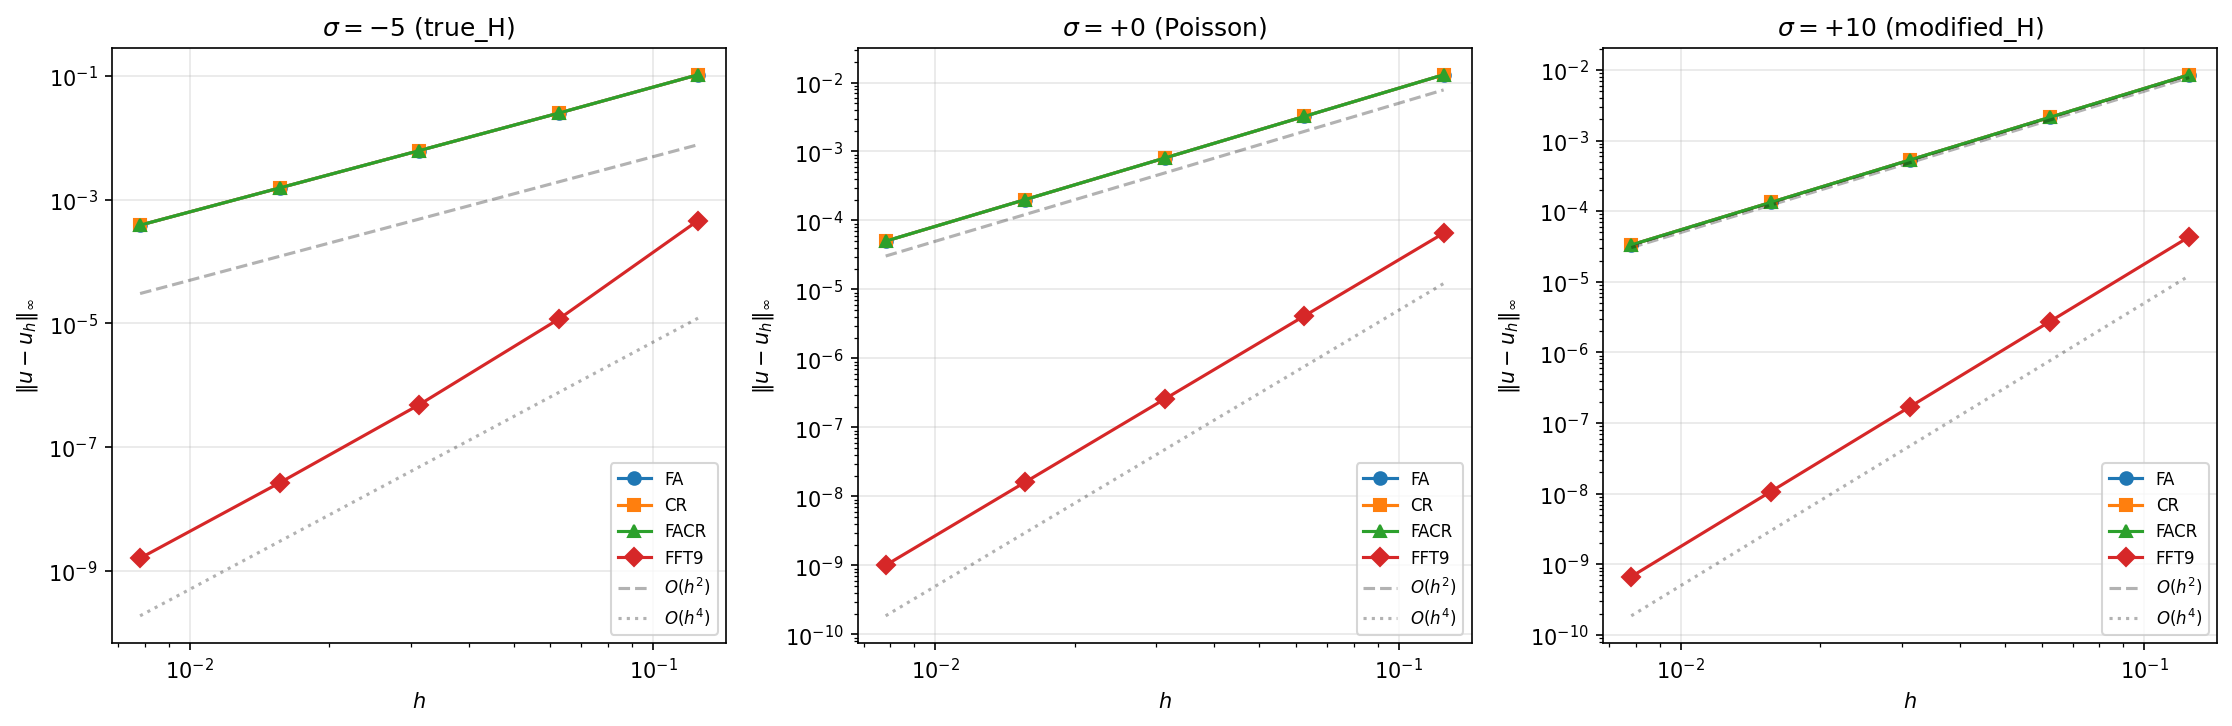
\includegraphics[width=0.82\textwidth]{figures/exp01_convergence.png}
\caption{二阶五点格式与四阶 FFT9 格式的收敛阶验证}
\label{fig:exp01_convergence}
\end{figure}

\begin{table}[htbp]
\centering
\caption{非特征多项式 manufactured solution 的收敛阶（$\sigma=10$）}
\label{tab:exp01_poly_convergence}
\begin{tabular}{cccc}
\toprule
方法 & $n$ & $L_\infty$ 误差 & 观测阶 \\
\midrule
FA / CR / FACR & 33  & $8.92\times10^{-6}$  & $2.00$ \\
FA / CR / FACR & 65  & $2.23\times10^{-6}$  & $2.00$ \\
FA / CR / FACR & 129 & $5.57\times10^{-7}$  & $2.00$ \\
FFT9           & 33  & $8.81\times10^{-9}$  & $4.00$ \\
FFT9           & 65  & $5.51\times10^{-10}$ & $4.00$ \\
FFT9           & 129 & $3.44\times10^{-11}$ & $4.00$ \\
\bottomrule
\end{tabular}
\end{table}

结果表明，FA、CR、FACR 对应的五点差分格式稳定呈现二阶精度，
FFT9 Dirichlet 紧致格式稳定呈现四阶精度。
该结论由 Fourier/Taylor 推导、模态测试和非特征多项式测试共同支撑。
本实验只验证离散格式收敛轨道，不用于判断 GMRES 迭代行为。

\subsection{实验三：非齐次 Dirichlet 边界条件验证}

本实验对应脚本 \texttt{exp02\_nonhom\_bc.py}。
取
\begin{equation}
  u(x,y)=\sin(2\pi x)\sin(3\pi y)+1,
\end{equation}
因此边界上 $g_D=1$，为真正的非齐次 Dirichlet 边界。
对应右端项为
\begin{equation}
  f(x,y)=\bigl((2\pi)^2+(3\pi)^2+\sigma\bigr)\sin(2\pi x)\sin(3\pi y)+\sigma.
\end{equation}
常数 $1$ 的 Laplacian 为零，因此不能写成
$((2\pi)^2+(3\pi)^2+\sigma)u(x,y)$。

\begin{figure}[htbp]
\centering
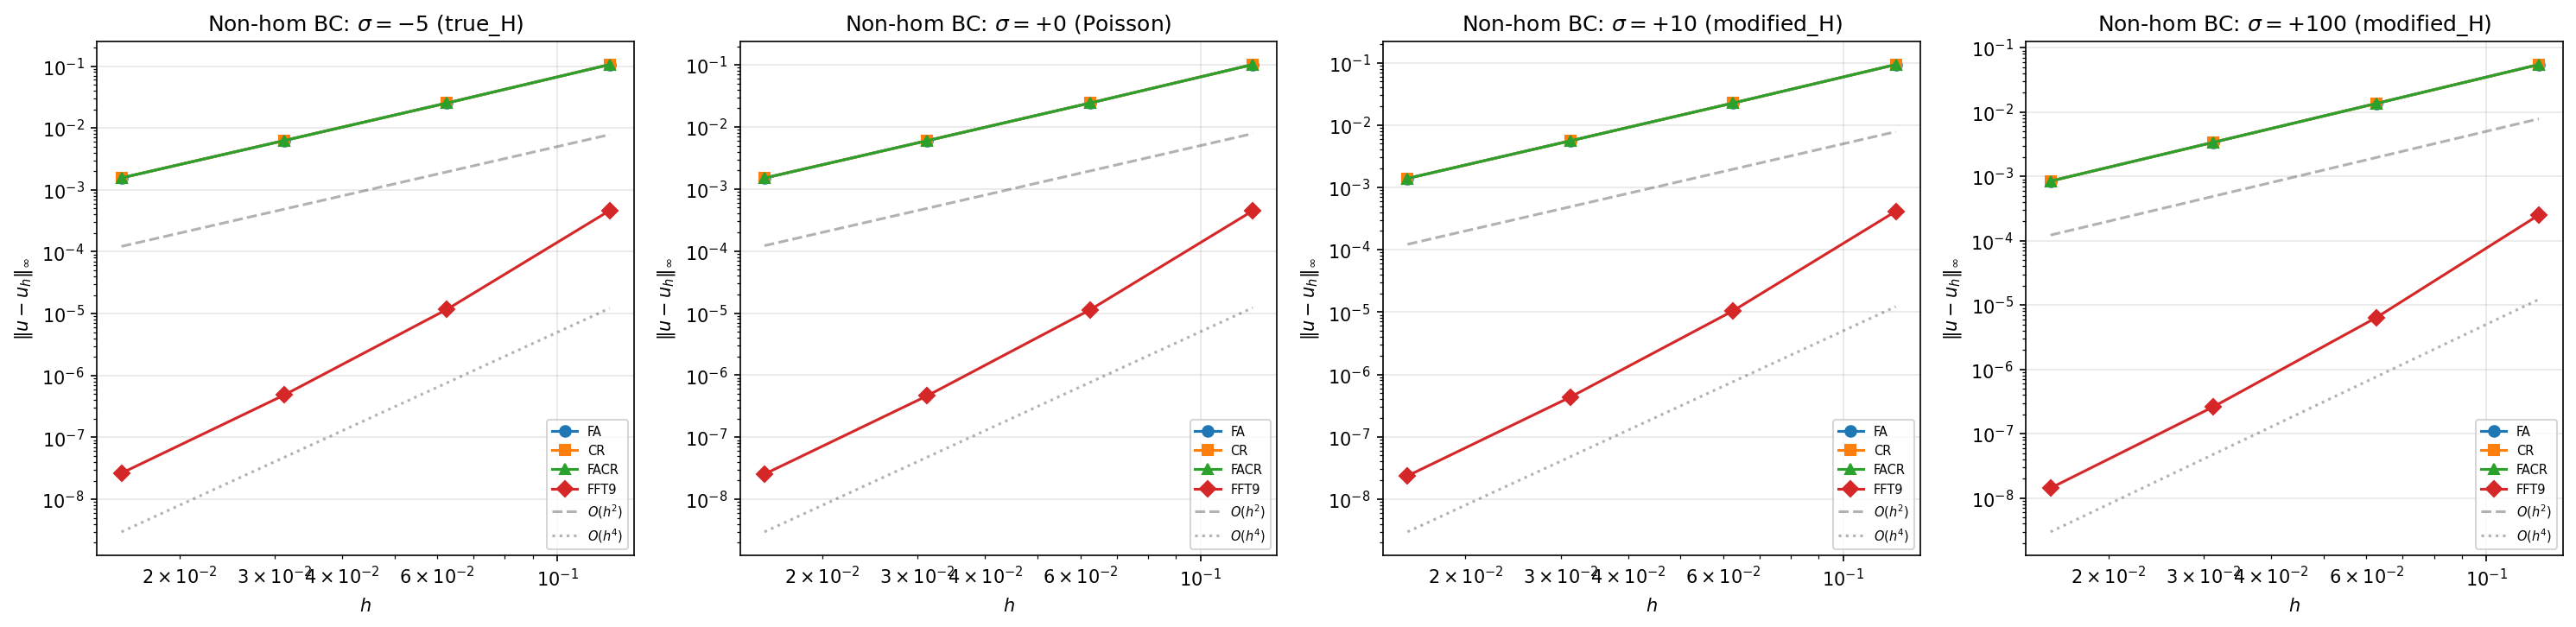
\includegraphics[width=0.82\textwidth]{figures/exp02_nonhom_bc.png}
\caption{非齐次 Dirichlet 边界条件下的误差收敛}
\label{fig:exp02_nonhom_bc}
\end{figure}

\begin{table}[htbp]
\centering
\caption{非齐次 Dirichlet 边界验证（$n=65$）}
\label{tab:exp02_nonhom_bc}
\begin{tabular}{ccccc}
\toprule
$\sigma$ & 方程类型 & 五点格式误差 & 五点格式阶 & FFT9 误差 / 阶 \\
\midrule
$0$    & Poisson     & $1.50\times10^{-3}$ & $2.00$ & $2.54\times10^{-8}$ / $4.19$ \\
$10$   & Modified H. & $1.39\times10^{-3}$ & $2.00$ & $2.36\times10^{-8}$ / $4.19$ \\
$100$  & Modified H. & $8.42\times10^{-4}$ & $2.00$ & $1.43\times10^{-8}$ / $4.19$ \\
$-5$   & True H.     & $1.56\times10^{-3}$ & $2.00$ & $2.64\times10^{-8}$ / $4.19$ \\
\bottomrule
\end{tabular}
\end{table}

表~\ref{tab:exp02_nonhom_bc} 说明，边界值移项符号修正后，
五点格式保持二阶收敛，FFT9 保持约四阶收敛。
这验证了非齐次 Dirichlet 情形下右端项和边界修正的实现一致性，
不涉及 Neumann 或混合边界的九点紧致格式推广。

\subsection{实验四：Neumann 与混合边界条件验证}

本实验对应脚本 \texttt{exp03\_neumann\_mixed.py}。
五点格式通过 ghost-point 方法和对称化 DCT-I/DST-I 组合处理 Neumann 与混合边界。
纯 Neumann Poisson 情形下，误差比较需去除常数偏移；
本文使用与 DCT-I 权重一致的 trapezoid-weighted mean。

\begin{figure}[htbp]
\centering
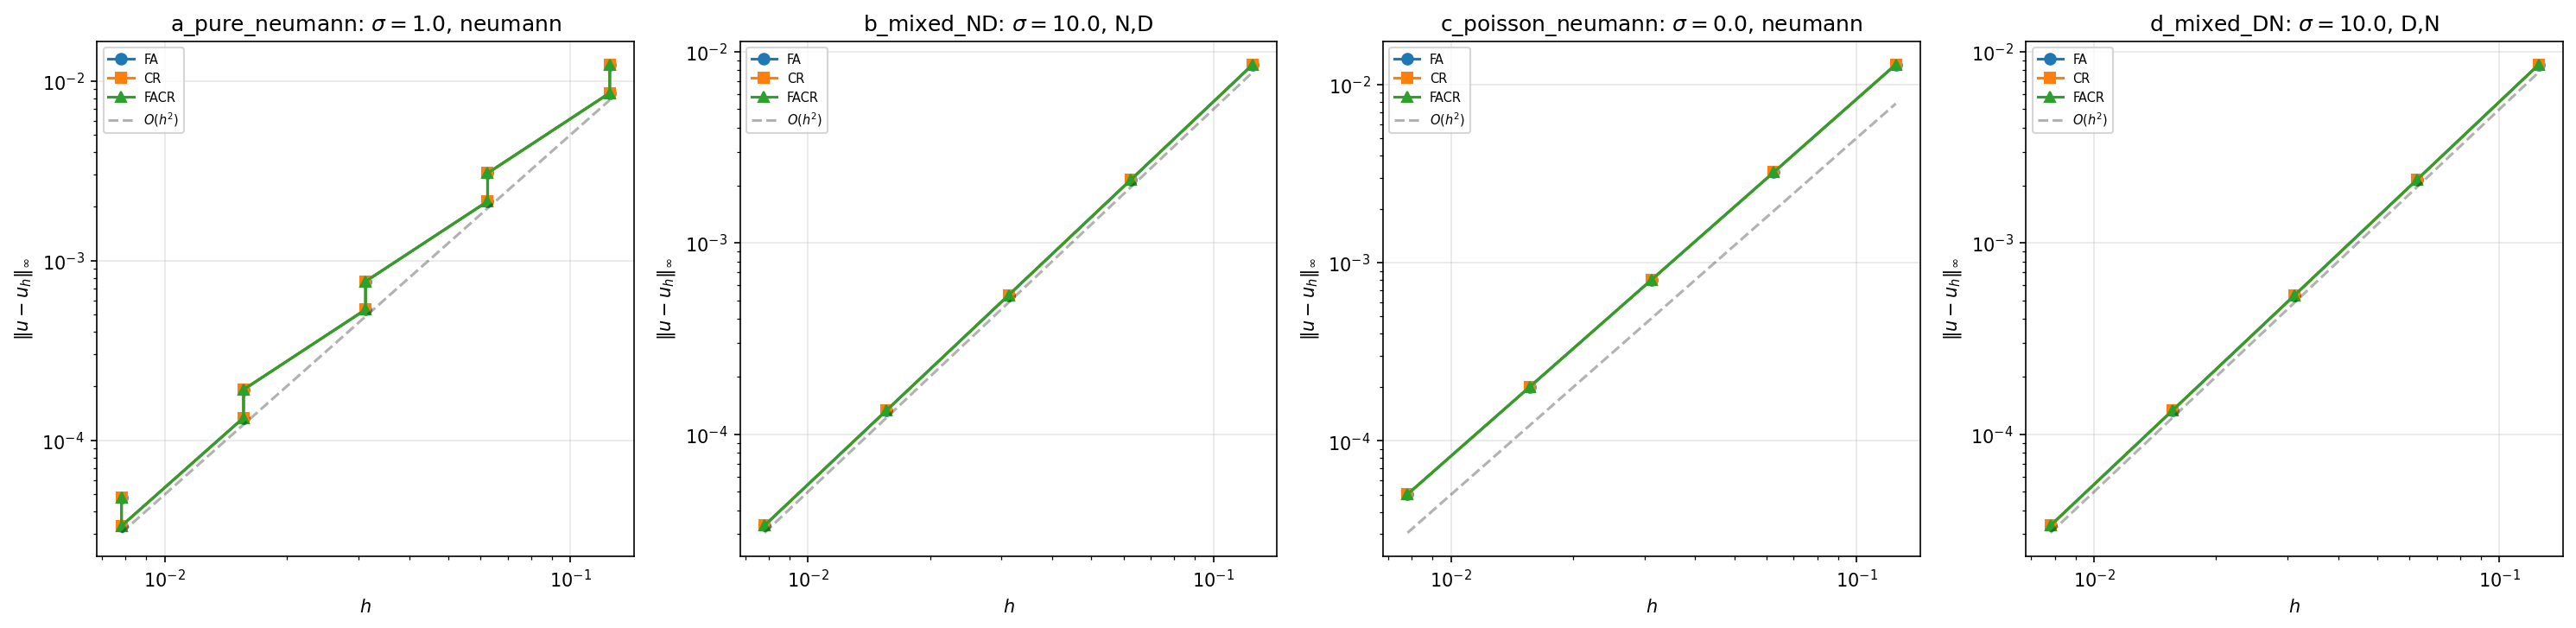
\includegraphics[width=0.82\textwidth]{figures/exp03_neumann_mixed.png}
\caption{Neumann 与混合边界条件下的收敛验证}
\label{fig:exp03_neumann_mixed}
\end{figure}

\begin{table}[htbp]
\centering
\caption{Neumann 与混合边界代表结果（FA，$n=65$）}
\label{tab:exp03_neumann_mixed}
\begin{tabular}{ccccc}
\toprule
子实验 & 边界类型 & $\sigma$ & $L_\infty$ 误差 & 观测阶 \\
\midrule
Pure Neumann & Neumann & $1$  & $1.91\times10^{-4}$ & $2.00$ \\
Pure Neumann & Neumann & $10$ & $1.33\times10^{-4}$ & $2.00$ \\
Mixed        & $(N,D)$ & $10$ & $1.33\times10^{-4}$ & $2.00$ \\
Neumann Poisson & Neumann & $0$ & $2.01\times10^{-4}$ & $2.00$ \\
Mixed        & $(D,N)$ & $10$ & $1.33\times10^{-4}$ & $2.00$ \\
\bottomrule
\end{tabular}
\end{table}

结果表明，ghost-point 对称化方法能够将 Neumann 和混合边界稳定纳入五点 FFT 框架。
需要注意的是，本实验不声称 FFT9 已支持 Neumann 或混合边界四阶格式；
FFT9 的四阶验证仅限 Dirichlet 边界。
因此，实验四验证的是受支持五点求解器的 Neumann/mixed 处理，不证明 FFT9 的 Neumann/mixed 四阶性。

\subsection{实验五：Modified 与 True Helmholtz 的谱指标和 GMRES 行为}

本实验对应脚本 \texttt{exp04\_modified\_vs\_true.py}。
谱指标由五点 Dirichlet 离散分母
\begin{equation}
  d_{p,q}=\lambda_{p,q}+\sigma
\end{equation}
给出。
当 $\sigma>0$ 时，modified Helmholtz 的分母恒正；
当 $\sigma<0$ 时，true Helmholtz 可能因 $-\sigma\approx\lambda_{p,q}$ 出现小分母和病态性。
GMRES 迭代实验使用 Gaussian 型非特征右端项
$f=\exp(-80((x-0.37)^2+(y-0.61)^2))$，
以避免单一 Fourier 模态造成的一步收敛退化。

\begin{figure}[htbp]
\centering
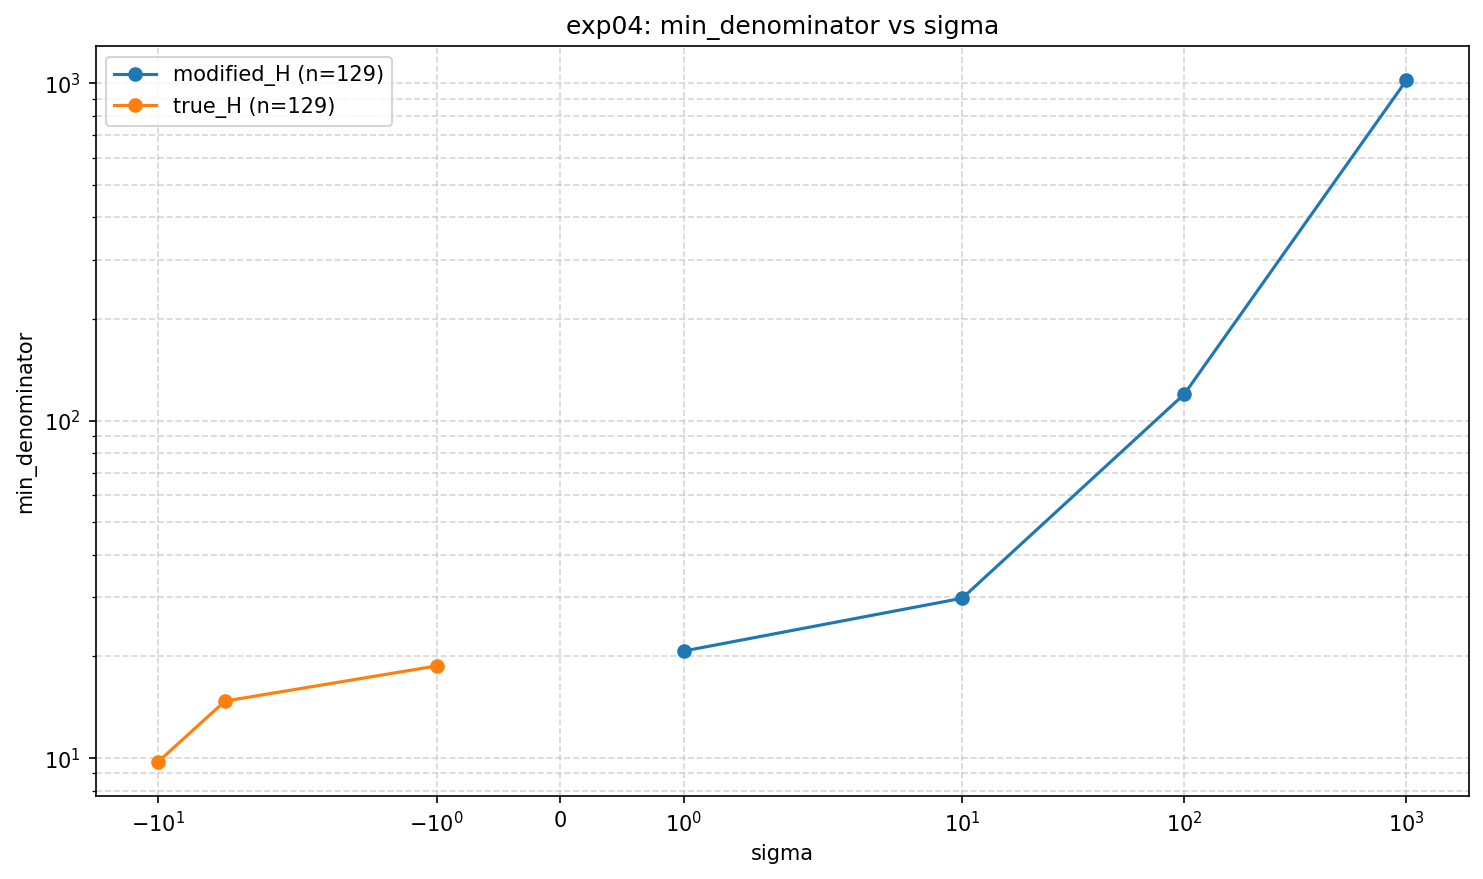
\includegraphics[width=0.48\textwidth]{figures/exp04_min_denom_vs_sigma.png}
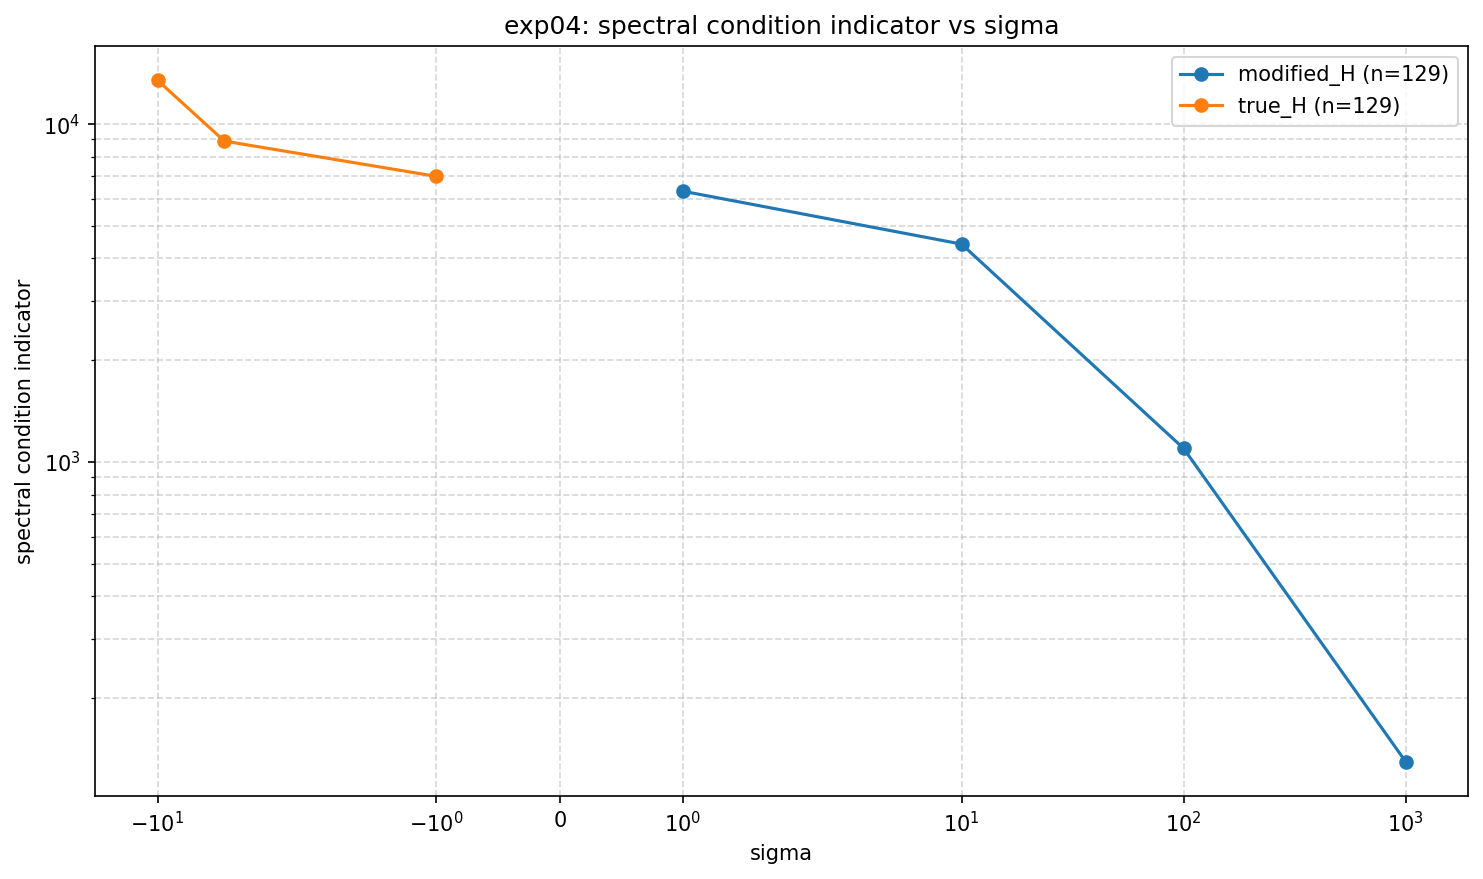
\includegraphics[width=0.48\textwidth]{figures/exp04_spectral_indicator_vs_sigma.png}
\caption{Modified/true Helmholtz 的最小频域分母与谱条件数指标}
\label{fig:exp04_spectral}
\end{figure}

\begin{figure}[htbp]
\centering
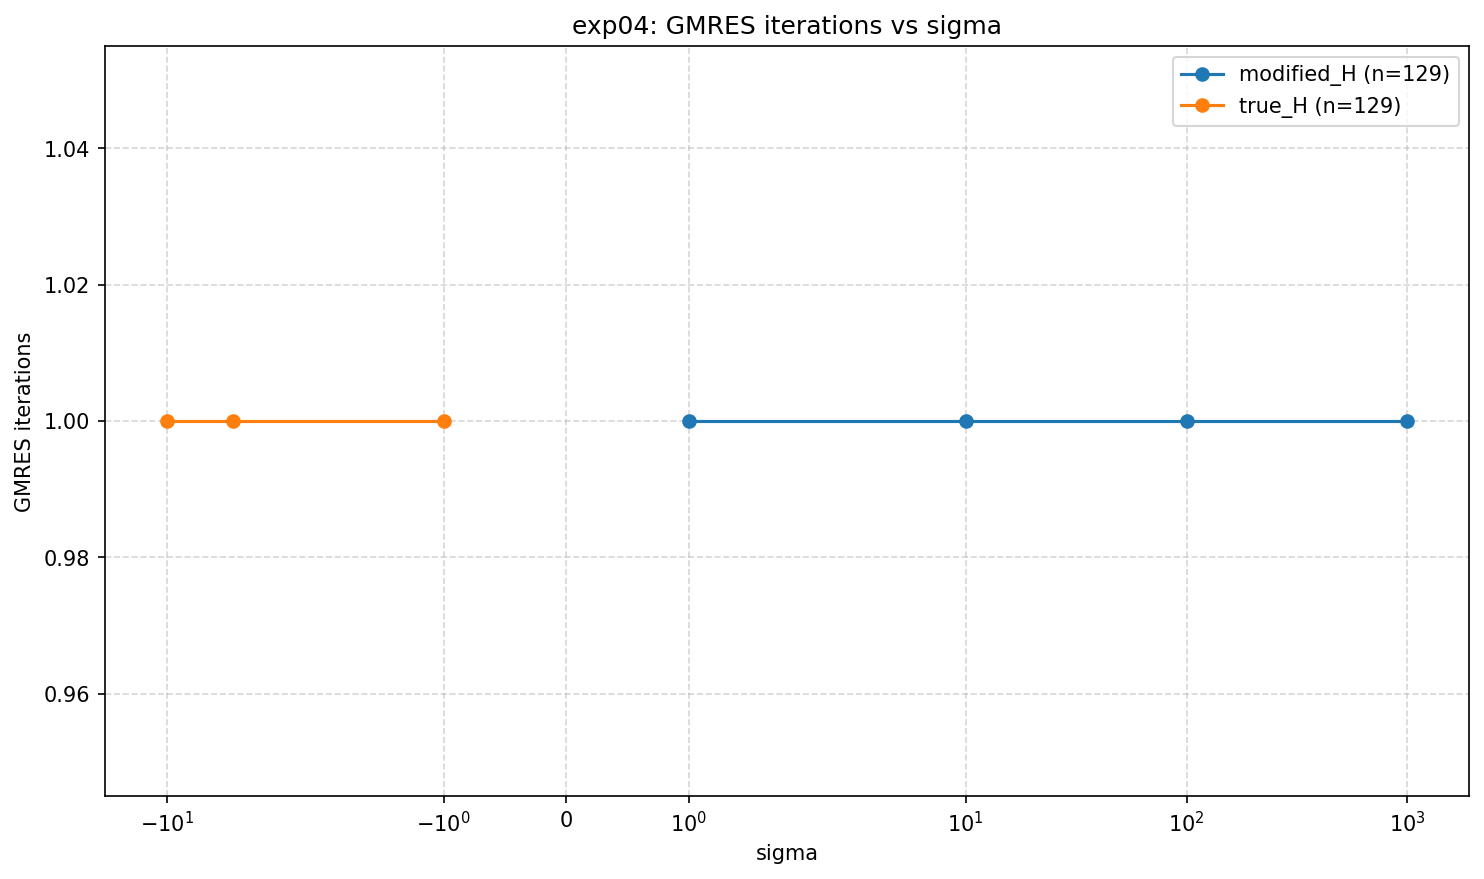
\includegraphics[width=0.68\textwidth]{figures/exp04_gmres_iters_vs_sigma.png}
\caption{Gaussian RHS 下无预处理 GMRES 迭代次数对比}
\label{fig:exp04_gmres}
\end{figure}

\begin{table}[htbp]
\centering
\caption{Modified/true Helmholtz 谱指标与 GMRES 迭代次数（$n=33$）}
\label{tab:exp04_mod_true}
\begin{tabular}{cccccc}
\toprule
$\sigma$ & 方程类型 & $d_{\min}$ & 谱指标 & GMRES 迭代 & 状态 \\
\midrule
$1$    & Modified & $20.72$ & $3.94\times10^2$ & $256$ & 收敛 \\
$10$   & Modified & $29.72$ & $2.75\times10^2$ & $203$ & 收敛 \\
$100$  & Modified & $119.72$ & $6.91\times10^1$ & $91$ & 收敛 \\
$1000$ & Modified & $1019.72$ & $8.99$ & $27$ & 收敛 \\
\midrule
$-1$   & True & $18.72$ & $4.36\times10^2$ & $270$ & 收敛 \\
$-5$   & True & $14.72$ & $5.55\times10^2$ & $319$ & 收敛 \\
$-10$  & True & $9.72$  & $8.39\times10^2$ & $428$ & 收敛 \\
$-50$  & True & $0.79$  & $1.03\times10^4$ & $>500$ & 近共振 \\
\bottomrule
\end{tabular}
\end{table}

表~\ref{tab:exp04_mod_true} 显示，modified Helmholtz 随 $\sigma$ 增大远离小分母，
谱指标改善，无预处理 GMRES 迭代次数下降；
true Helmholtz 随 $|\sigma|$ 接近离散 Laplacian 特征值而出现小分母风险，
GMRES 迭代变慢甚至在给定上限内未收敛。
该实验只观察 Gaussian RHS 下无预处理 GMRES 的参数敏感性，不构成完整迭代法性能研究。

\subsection{实验六：True Helmholtz 近共振扫描}

本实验对应脚本 \texttt{exp05\_true\_helmholtz\_resonance.py}。
取 $n=65$，目标模态 $(p,q)=(2,1)$，
离散特征值 $\lambda_{2,1}^h\approx49.3143$，
令
\begin{equation}
  \sigma=-(\lambda_{2,1}^h+\delta),
\end{equation}
并扫描正负两侧的小扰动 $\delta$。
右端项仍采用 Gaussian 型非特征函数。

\begin{figure}[htbp]
\centering
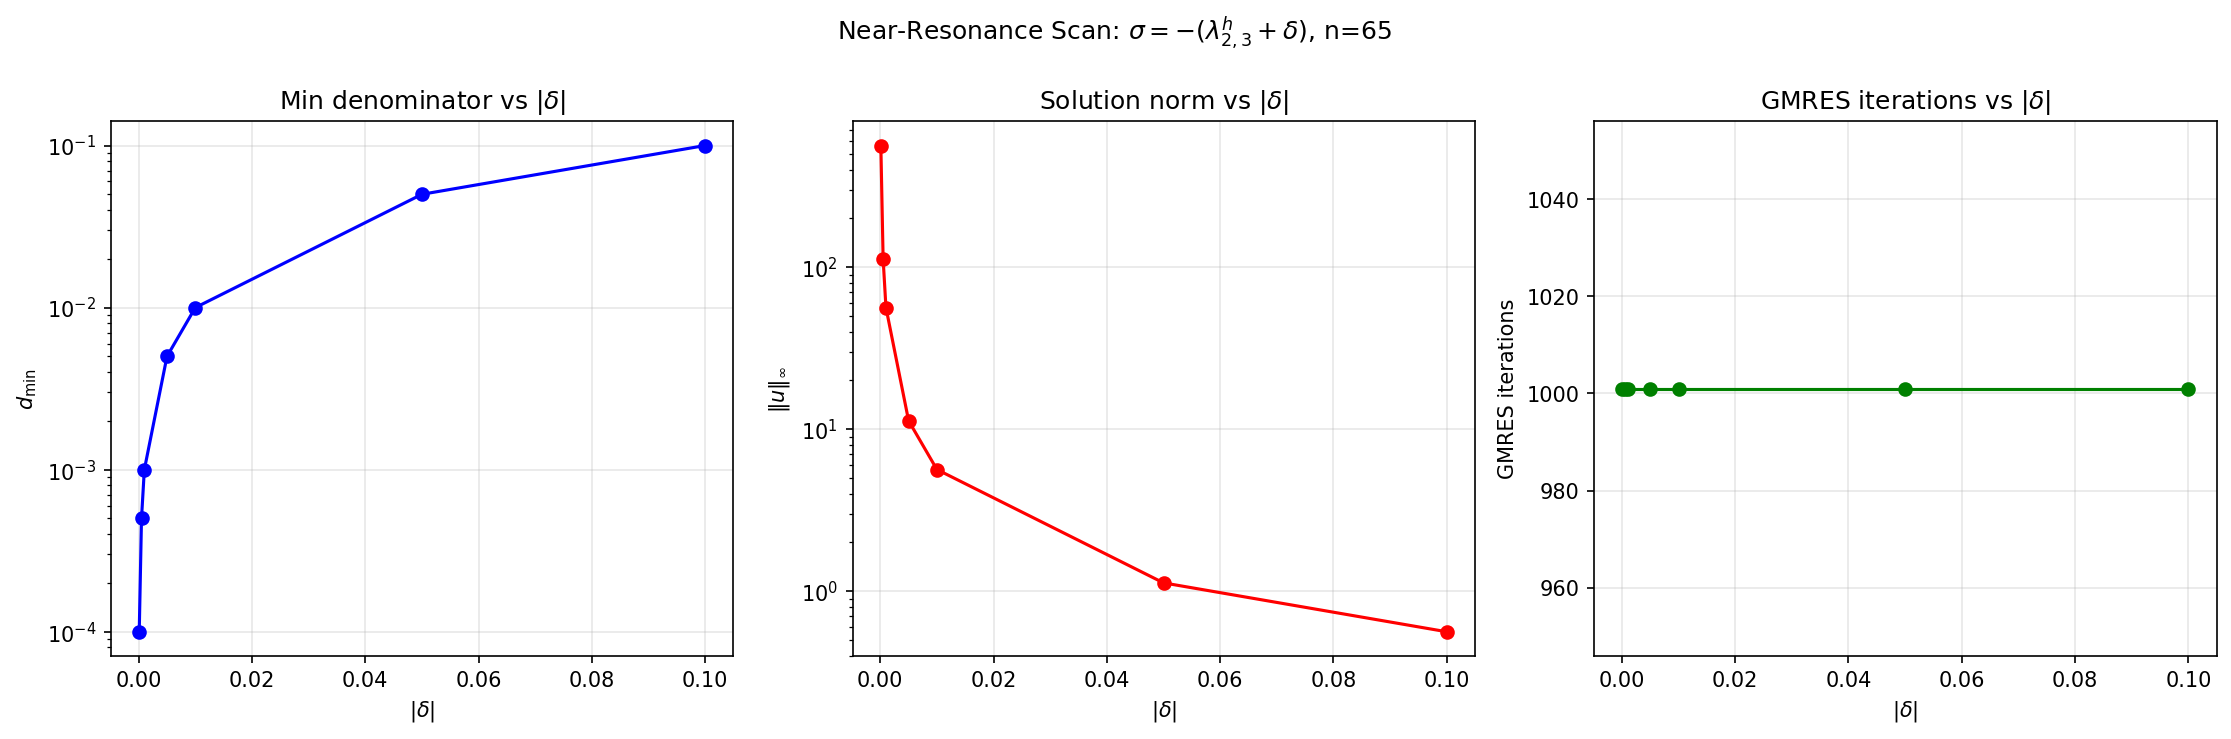
\includegraphics[width=\textwidth]{figures/exp05_resonance.png}
\caption{True Helmholtz 近共振扫描：$d_{\min}$、解范数和 GMRES 迭代随 $|\delta|$ 的变化}
\label{fig:exp05_resonance}
\end{figure}

\begin{table}[htbp]
\centering
\caption{近共振扫描代表数据（$n=65$）}
\label{tab:exp05_resonance}
\begin{tabular}{cccc}
\toprule
$|\delta|$ & $d_{\min}$ & $\|u\|_\infty$ & GMRES 迭代 \\
\midrule
$10^{-1}$ & $1.00\times10^{-1}$ & $1.32$ & $1001$（未收敛） \\
$10^{-2}$ & $1.00\times10^{-2}$ & $13.19$ & $1001$（未收敛） \\
$10^{-3}$ & $1.00\times10^{-3}$ & $131.92$ & $1001$（未收敛） \\
$10^{-4}$ & $1.00\times10^{-4}$ & $1.32\times10^{3}$ & $1001$（未收敛） \\
\bottomrule
\end{tabular}
\end{table}

结果验证了第\ref{sec:helmholtz}章的频域分析：
当 $\kappa^2$ 接近离散 Laplacian 特征值时，最小分母 $d_{\min}$ 下降，
对应模态的解分量被放大，线性系统变得病态。
无预处理 GMRES 在这些近共振参数下无法在给定迭代上限内收敛，
说明 true Helmholtz 问题通常需要 shifted-Laplacian 等预处理技术。
该结论仅针对 true Helmholtz 近共振扫描，不外推为一般波数性能比较。

\subsection{实验总结}

本章将原有大量历史实验压缩为六组可复现的核心实验。
实验一验证 FFT 类五点求解器与稀疏直接解的一致性；
实验二验证五点格式二阶和 FFT9 Dirichlet 紧致格式四阶；
实验三验证非齐次 Dirichlet 右端项与边界修正符号；
实验四验证 Neumann 与混合边界在五点 FFT 框架中的处理；
实验五和实验六分别从远离共振的谱指标和近共振扫描两方面说明 modified/true Helmholtz 的本质差异。

由这些实验可得：
\begin{itemize}[itemsep=2pt]
  \item 对规则单位正方形和均匀网格，FFT 直接法能够高精度求解对应离散系统；
  \item 五点格式和 FFT9 Dirichlet 紧致格式分别呈现二阶和四阶精度；
  \item 非齐次 Dirichlet、Neumann 与混合边界的实现已通过离散一致性或收敛阶验证；
  \item modified Helmholtz 与 true Helmholtz 的差异来自频域分母结构，不能把二者的迭代行为混写；
  \item true Helmholtz 在近共振时出现解范数放大和无预处理 GMRES 收敛困难。
\end{itemize}

本章不再保留无统计重复计时、装饰性热力图、GMRES 重启参数图或单独复杂度趋势图作为核心证据。
这些材料可作为探索性输出留存在图像目录中，但不参与本文最终结论。

% ============================================================
% 第七章 结论与展望
% ============================================================
\section{结论与展望}
\label{sec:conclusion}

\subsection{本文工作总结}

本文针对矩形区域上的 Poisson 方程和 Helmholtz 方程，
系统研究了基于 FFT 的快速直接求解方法，并与 GMRES 迭代法进行了对比分析。
主要工作和贡献如下：

\begin{enumerate}
  \item \textbf{FFT 快速直接求解器族}：实现了基于离散正弦/余弦变换的五种快速求解器
        ——FA（Fourier Analysis）、CR（Cyclic Reduction）、FACR（混合算法）、
        FFT9（四阶紧致差分）和五点差分直接法。
        其中 FACR 算法通过结合 CR 和 FA 的优势，
        实现了 $O(N^2 \log\log N)$ 的最优时间复杂度。

  \item \textbf{Helmholtz 方程扩展}：通过 $k^2$ 修正将 Poisson 求解器自然推广到
        Helmholtz 方程 $(-\nabla^2 + k^2)u = f$，
        并分析了共振条件 $\lambda_p + \lambda_q + k^2 = 0$ 对求解的影响。

  \item \textbf{Neumann 边界条件的 ghost-point 对称化方法}：
        针对 Neumann 边界条件导致的 Laplacian 矩阵非对称问题，
        提出了 ghost-point 方法配合对称化 DCT-I 变换的解决方案。
        通过对角缩放矩阵 $D = \mathrm{diag}(\sqrt{2}, 1, \ldots, 1, \sqrt{2})$
        将非对称矩阵 $G$ 对称化为 $S = D^{-1}GD$，
        使其被 DCT-I 对角化，从而在 FFT 框架内统一处理 Dirichlet 和 Neumann 边界条件。

  \item \textbf{六阶格式不可行的证明}：通过 Fourier 特征值分析严格证明了，
        对于九点紧致差分格式的三参数修正族
        $(L_h + \alpha h^2 L_h^{(5)})u - k^2(R_h+\beta h^2 I)u = -(R_h+\gamma h^2 I)f$，
        不存在统一的常数 $(\alpha, \beta, \gamma)$ 使得截断误差达到 $O(h^6)$。
        具体地，在 Poisson 方程情形下，$c_2 = 0$ 要求 $\alpha = -\gamma$，
        但 $c_4(1,0,\gamma) = 0$ 要求 $\gamma = -1/20$，
        而 $c_4(1,1,\gamma) = 0$ 要求 $\gamma = 1/30$，
        两者矛盾（$2(60\gamma+3)-(120\gamma-4) = 10 \neq 0$）。
        该结论已在 Lean 4 定理证明器中完成形式化验证（整数域 12 定理 + 实数域 5 定理）。
        在 Helmholtz 方程（$k^2 \neq 0$）情形下，连 $c_2 = 0$ 都无法统一满足，
        即不存在使 $O(h^2)$ 误差项消失的通用参数。

  \item \textbf{GMRES 迭代法对比}：实现了基于 Givens 旋转的 GMRES(m) 算法，
        构造了二维 Helmholtz 方程的五点差分稀疏矩阵，
        在相同测试问题下与 FFT 直接法进行了系统的精度、效率和收敛性对比。
        数值实验表明，FFT 直接法在规则区域上具有显著的效率优势。
\end{enumerate}

\subsection{主要结论}

\begin{enumerate}
  \item 在规则矩形区域上，FFT 直接法是求解 Poisson/Helmholtz 方程的首选方法。
        FA 方法实现简单、效率高；FACR 方法在细网格下具有最优复杂度；
        FFT9 方法以适度的额外计算量换取四阶精度。

  \item GMRES 迭代法在规则区域上的效率不如 FFT 直接法，
        但具有更好的通用性——它可以处理非均匀网格、
        变系数问题和复杂几何区域，这些是 FFT 直接法难以处理的。

  \item 波数 $k$ 对求解效果有显著影响：
        FFT 直接法对波数不敏感（只要避开共振），
        而 GMRES 的迭代次数随波数增大而显著增加，
        反映了 Helmholtz 方程在大波数下的固有困难。

  \item Ghost-point 对称化 DCT-I 方法是处理 Neumann 边界条件的一种优雅方案，
        它将 Neumann 问题无缝纳入 FFT 直接法框架，
        保持了方法的统一性和高效性。
\end{enumerate}

\subsection{展望}

本文的研究可以在以下方向进一步拓展：

\begin{enumerate}
  \item \textbf{非均匀网格}：当前方法基于均匀网格。
        对于解变化剧烈的区域，自适应网格加密技术（如 FAC 方法）
        可以在保持精度的同时减少计算量。
        如何将 FFT 快速求解器与非均匀网格结合是一个有价值的研究方向。

  \item \textbf{变系数问题}：当方程系数（如介质参数）空间变化时，
        FFT 直接法不再适用，此时迭代法（配合适当的预处理）成为主要选择。
        研究基于 FFT 的高效预处理子是一个重要的课题。

  \item \textbf{高维问题}：本文的方法可以自然推广到三维问题。
        三维问题的 FFT 直接法复杂度为 $O(N^3 \log N)$，
        而 FACR 可以达到 $O(N^3 \log\log N)$，
        但内存需求随维数快速增长，需要更高效的实现策略。

  \item \textbf{大规模 Helmholtz 问题}：对于高频（大波数）Helmholtz 方程，
        GMRES 的收敛性严重依赖于预处理的质量。
        研究基于 Shifted Laplacian 的预处理方法、
        多层方法（Multigrid）以及区域分解方法，
        是解决大规模 Helmholtz 问题的前沿方向~\cite{Ernst2011, YaoDengming2018, Niu2009}。
        此外，物理信息神经网络（PINN）等新兴方法~\cite{ShanLianpu2023}
        也为 Helmholtz 方程的求解提供了新思路。

  \item \textbf{形式化验证}：本文对六阶不可行定理进行了 Lean 4 形式化验证，
        这是将交互式定理证明器应用于数值分析领域的一次尝试。
        未来可以将形式化验证扩展到更广泛的差分格式理论，
        如稳定性分析（Lax 等价定理）、收敛阶估计等，
        为数值算法的可靠性提供机器可验证的数学保证。

  \item \textbf{GPU 加速}：FFT 和稀疏矩阵-向量乘法都适合在 GPU 上并行执行。
        利用 CUDA 或 OpenCL 实现 GPU 加速版本，
        可以将求解速度提升一到两个数量级，
        使其能够处理更大规模的实际问题。
\end{enumerate}


% ============================================================
% 附录
% ============================================================
\newpage
\appendix
% ============================================================
% 附录：Lean 4 辅助形式化验证
% ============================================================
\section{Lean 4 辅助形式化验证}
\label{app:lean4}

本文使用 Lean 4 辅助验证三参数九点修正族六阶 local consistency 不可达性反证中的代数核心。
验证对象不是完整 PDE 收敛定理，而是 local Fourier symbol 展开后得到的有限个多项式系数条件。

\subsection{验证目标}

考虑定理~\ref{thm:6th_impossible}中的三参数九点修正族：
\begin{equation}
  (-L_h - \alpha h^2 L_h^{(5)})u + \sigma(R_h+\beta h^2 I)u = (R_h+\gamma h^2 I)f,
\end{equation}
其中 $\alpha,\beta,\gamma$ 是与 Fourier mode 无关的统一常数。
在 local Fourier symbol 展开中，六阶一致性要求 $h^2$ 项系数 $c_2$ 和
$h^4$ 项系数 $c_4$ 对所有连续波数同时为零。Lean 4 辅助验证的目标是检查这些
系数条件中的有限代数核心：
\begin{enumerate}[itemsep=1pt]
  \item \(c_2=0\) 推出的参数必要关系；
  \item 代入这些必要关系后，两个 Fourier 测试模式对应的 \(c_4=0\) 条件互相矛盾；
  \item 因此不存在统一实数参数使这些必要条件同时成立。
\end{enumerate}

\subsection{验证定理与策略}

表~\ref{tab:lean4_theorems} 列出了 Lean 4 中验证的核心实数域定理。
该表只对应反证链条中的有限个代数命题，不表示从差分模板到 PDE 全局误差估计的完整形式化。
\begin{table}[H]
\centering
\caption{Lean 4 辅助验证的代数核心定理清单}
\label{tab:lean4_theorems}
\resizebox{\textwidth}{!}{%
\begin{tabular}{llll}
\toprule
\textbf{Lean 定理名} & \textbf{数学含义} & \textbf{证明策略} & \textbf{状态} \\
\midrule
\texttt{c4\_num\_mode\_10\_real} & \(c_4(1,0,\gamma)=60\gamma+3\) 的代数展开 & \texttt{ring} & 通过 \\
\texttt{c4\_num\_mode\_11\_real} & \(c_4(1,1,\gamma)=120\gamma-4\) 的代数展开 & \texttt{ring} & 通过 \\
\texttt{sixth\_order\_impossible\_real} & 两个测试模式的 \(c_4=0\) 条件不相容 & \texttt{ring}+\texttt{linarith} & 通过 \\
\texttt{c2\_poisson\_forces\_neg\_gamma} & Poisson 情形下 \(c_2=0\) 推出必要关系 \(\alpha=-\gamma\) & \texttt{linarith} & 通过 \\
\texttt{poisson\_no\_sixth\_order\_real} & Poisson 三参数族的 local symbol 六阶条件不相容 & \texttt{ring}+\texttt{linarith} & 通过 \\
\texttt{c2\_helmholtz\_forces\_neg\_gamma} & Helmholtz 情形下 \(c_2=0\) 推出必要关系 \(\alpha=-\gamma\) & \texttt{linarith} & 通过 \\
\texttt{helmholtz\_no\_sixth\_order\_real} & Helmholtz 三参数族的 local symbol 六阶条件不相容 & \texttt{ring}+\texttt{linarith} & 通过 \\
\bottomrule
\end{tabular}%
}
\end{table}

表中定理只对应反证中的代数步骤。它们说明：一旦 \(c_2=0\) 给出必要参数关系，
两个测试波数 \((1,0)\) 与 \((1,1)\) 的 \(c_4=0\) 条件就无法由同一个常数
\(\gamma\) 同时满足。
这里的 \((1,0)\) 与 \((1,1)\) 是 local Fourier symbol 中的连续波数测试点，
不是 Dirichlet DST-I 离散模态编号。
其中，\texttt{c2\_helmholtz\_forces\_neg\_gamma} 直接验证的是
Helmholtz 情形下 \(c_2=0\) 所需参数关系中的 \(\alpha=-\gamma\) 代数核心；
若在论文推导中使用 \(\beta=\gamma\)，该关系来自相应系数方程的纸面推导，
而不是该 Lean 定理的直接结论。

\subsection{验证范围与局限性}

\textbf{已验证的内容}：
\begin{enumerate}[itemsep=1pt]
  \item \(c_4\) 系数在测试波数 \((1,0)\) 和 \((1,1)\) 上的显式代数表达式；
  \item 两个测试波数的 \(c_4=0\) 条件互相矛盾；
  \item \(c_2=0\) 推出相应参数必要关系的代数步骤；
  \item Poisson 与 Helmholtz 两种情形中 \(c_2 \to c_4\) 反证路径的代数不相容性。
\end{enumerate}

\textbf{未覆盖的内容}：
\begin{enumerate}[itemsep=1pt]
  \item Fourier symbol 从差分模板导出的全过程；
  \item Taylor 展开建模为 \(c_2,c_4\) 的全过程；
  \item Dirichlet DST-I 谱理论或 Neumann/Mixed 边界下的 DCT 理论；
  \item 边界闭合分析；
  \item 完整 PDE 全局误差估计；
  \item Python 求解器、实验脚本或数值实验结果的程序正确性。
\end{enumerate}

\subsection{形式化验证工具链}

\begin{itemize}[itemsep=2pt]
  \item \textbf{Lean 版本}：leanprover/lean4:v4.29.1
  \item \textbf{Mathlib 版本}：v4.29.1（预编译 olean）
  \item \textbf{构建命令}：\texttt{lake build}
  \item \textbf{验证状态}：自有形式化文件无 \texttt{sorry}、\texttt{admit}、\texttt{axiom} 或 \texttt{unsafe}，全部定理通过编译。
\end{itemize}

\begin{remark}
  Lean 4 验证覆盖的是 Fourier symbol 展开之后的有限多项式条件之间的不相容性，
  为论文中的代数反证提供机器可检查的支持。
  它不声称证明完整 PDE 收敛理论、边界闭合理论、DST/DCT 谱理论或 Python 程序正确性。
\end{remark}


% ============================================================
% 参考文献
% ============================================================
\bibliographystyle{unsrt}
\bibliography{references}

% ============================================================
% 致谢
% ============================================================
\newpage
\section*{致谢}
\addcontentsline{toc}{section}{致谢}

感谢导师在论文选题和研究过程中的悉心指导，感谢同学在数值实验中的讨论与帮助。

\end{document}
